\title{Fitting a Quantile Regression Model for Residual Life with the R Package qris}
\author{Kyu Hyun Kim, Sangwook Kang, and Sy Han Chiou}

\maketitle

\abstract{
  In survival analysis, regression modeling has traditionally focused on assessing covariate effects on survival times, 
  which is defined as the elapsed time between a baseline and event time. 
  Nevertheless, focusing on residual life can provide a more dynamic assessment of covariate effects, 
  as it offers more updated information at specific time points between the baseline and event occurrence.
  Statistical methods for fitting quantile regression models have recently been proposed, 
  providing favorable alternatives to modeling the mean of residual lifetimes. 
  Despite these progresses, the lack of computer software that implements these methods remains an obstacle for researchers analyzing data in practice. 
  In this paper, we introduce an R package \CRANpkg{qris} \citep{R:qris}, which implements methods for fitting semiparametric quantile regression models on residual life subject to right censoring.
  We demonstrate the effectiveness and versatility of this package through comprehensive simulation studies and 
  a real-world data example, showcasing its valuable contributions to survival analysis research.
}

\section{Introduction} \label{sec:intro}

In the analysis of time-to-event data, standard statistical inference procedures often focus on quantities 
based on failure time and its relationship with covariates measured at baseline. 
However, throughout the follow-up process,
inference procedures based on residual life become increasingly intuitive for assessing the survival of subjects 
and can offer insights into the effectiveness of treatments in prolonging the remaining lifetime. 
As covariates can substantially change over time and
models based solely on baseline covariates have limited potential for long-term prognosis, 
there is a growing interest in modeling the remaining lifetime of a surviving subject with updated patient information. 
Many efforts have been made to model the mean residual life including proportional mean residual life models 
\citep{maguluri1994estimation, oakes1990note, oakes2003inference, chen2005semiparametric}, 
additive mean residual life models \citep{chen2006linear, chen2007additive, zhang2010goodness}, 
and proportional scaled mean residual life models \citep{liu2008regression}. 
Given that failure times are usually right-skewed and heavy-tailed, 
the mean of the residual life might not be identifiable if 
the follow-up time is not sufficiently long. 
For this reason, quantiles, which are robust under skewed distribution, 
have traditionally been used more frequently as alternative summary measures.
For example, the approach on the semiparametric quantile regression model for continuous responses \citep{koenker1978regression} has been extended to uncensored failure time data 
\citep{jung1996quasi, portnoy1997gaussian, wei2006quantile} 
and censored failure times data \citep{ying1995survival, portnoy2003censored,peng2008survival, huang2010quantile}. 


When the outcome variable is the residual life, 
semiparametric quantile models that apply the inverse probability of censoring weighting (IPCW) 
principle to address right-censored observations have been explored 
\citep{jung2009regression, kim2012censored, li2016quantile}.
These approaches are based on non-smooth estimating functions with respect to regression parameters, 
and the estimates of the regression parameters are obtained either through zero-crossing of 
non-smooth estimating functions using grid search techniques \citep{jung2009regression} or 
by optimizing non-smooth objective functions with $L_1$-minimization algorithms \citep{kim2012censored, li2016quantile}. 
While these methods are relatively straightforward to implement, 
an additional challenge lies in standard error estimation, 
which necessitates the computationally intensive use of a multiplier bootstrap method \citep{li2016quantile}.
Alternatively, \citet{jung2009regression} and \citet{kim2012censored} utilized the minimum dispersion statistic and 
the empirical likelihood method, respectively, 
to bypass the need to directly estimate the variance of the regression parameter estimator for 
hypothesis testing and constructing confidence intervals.
The non-smooth nature of the estimating functions in these approaches 
precludes the estimation of variance using the robust sandwich-type variance estimator typically employed 
in equation-based estimation methods. 
To lessen the associated computational burden, an induced smoothing was proposed \citep{brown2005standard}, 
which modifies the non-smooth estimating equations into smooth ones.
Leveraging the asymptotic normality of the non-smooth estimator, 
the smooth estimating functions are constructed by averaging out the random perturbations 
inherent in the non-smooth estimating functions.
The resulting estimating functions become smooth with respect to the regression parameters, 
allowing for the straightforward application of standard numerical algorithms, such as the Newton-Raphson method.
Furthermore, these smoothed estimating functions facilitate the straightforward computation of variances using 
the robust sandwich-type estimator.
The induced smoothing approach has been employed in fitting semiparametric accelerated failure time (AFT) models 
via the rank-based approach \citep{johnson2009induced, aftgeepackage, chiou2015semiparametric, Kang:fitt:2016}.
Regarding quantile regression, \citet{choi2018smoothed} considered the induced smoothing approach under 
a competing-risks setting. All of these methods are based on modeling event times.
Recently, \citet{kim2023smoothed} proposed an induced smoothing estimator for fitting 
a semiparametric quantile regression model for residual life.



The availability of published R packages for fitting quantile regression models is somewhat limited. 
The \code{rq()}, \code{nlrq()}, \code{rqss()}, and \code{crq()} functions in the package \CRANpkg{quantreg} 
\citep{quantregpackage} are predominantly used and provide various features for fitting linear, 
nonlinear, non-parametric, and censored quantile regression models, respectively.
The \code{rq()} function minimizes non-smooth objective functions to obtain point estimates of regression coefficients 
and can accommodate right-censored survival times by incorporating weights.
By redefining survival times as the remaining lifetime at time $t_0$, 
one can also obtain a non-smoothed estimator for quantile regression models for residual life \citep{kim2012censored}.
On the other hand, the \code{nlrq()} function is designed to fit a nonlinear quantile regression model, while
the \code{rqss()} function fits additive quantile regression models with 
nonparametric terms, including univariate components and bivariate components, 
using smoothing splines and total variation regularization techniques \citep{koenker1994quantile, koenker2004penalized}.
% On the other hand, the \code{nlrq()} function is designed to fit a nonlinear quantile regression model, 
% while the \code{rqss()} function fits additive quantile regression models with nonparametric terms, 
% including univariate components and bivariate components, using smoothing splines and 
% total variation regularization techniques \citep{koenker1994quantile, koenker2004penalized}.
Furthermore, the \code{crq()} function fits a quantile regression model for censored data on the $\tau$-th 
conditional quantile function of the response variable.
Overall, the \CRANpkg{quantreg} implements three methods for handling right-censored survival times: \citet{powell1986censored}'s estimator,
\citet{portnoy2003censored}'s estimator and \citet{peng2008survival}'s estimator. 
However, none of the implemented methods in the \code{nlrq()}, \code{rqss()}, or \code{crq()} functions 
are applicable for handling censored residual life using the induced smoothing methods. 
The only function that implements the induced smoothing method is the \code{aftsrr()} function in the package 
\CRANpkg{aftgee} \citep{aftgeepackage}, 
but it is specifically designed for fitting semiparametric AFT models, which are not directly applicable 
to fitting quantile regression models.


% In an effort to lessen the computational burden in handling non-smooth estimating equations,
% the \code{aftsrr()} function in package \CRANpkg{aftgee} \citep{aftgeepackage} is the only function that implements the induced smoothing method in the context of fitting semiparametric AFT models. 

Other R packages that can be used to fit quantile regression models for survival data include the package 
\CRANpkg{ctqr} \citep{ctqrpackage}, package \CRANpkg{Brq} \citep{Brqpackage}, package \CRANpkg{brms} \citep{brmspackage}, 
and package \CRANpkg{cmprskQR} \citep{cmprskQRpackage}.
The \code{ctqr()} function in the package \CRANpkg{ctqr} implements the methods proposed in 
\citet{ctqrpackage} for right or interval-censored failure times with left-truncation.
The \code{Bqr()} function in the package \CRANpkg{Brq} implements Bayesian methods based on the 
asymmetric Laplace distribution.
In the package \CRANpkg{brms}, the \code{brm()} function with the \code{family=asym\_laplace()} 
option enables the implementation of full Bayesian inference.
The \code{crrQR()} function in the package \CRANpkg{cmprskQR} allows fitting quantile regression models 
with competing risks.
All of these R packages are designed for fitting quantile regression models for failure times defined from a baseline 
and are not applicable to the residual life setting.

% In an effort to lessen the computational burden in handling non-smooth estimating equations,
% the \code{aftsrr()} function in package \CRANpkg{aftgee} \citep{aftgeepackage} is the only function that implements the induced smoothing method in the context of fitting semiparametric AFT models. 

The recently developed R package \CRANpkg{qris} \citep{R:qris} provides an efficient tool for 
fitting semiparametric quantile regression models for residual life subject to right censoring.
The \CRANpkg{qris} package offers three methods for estimating the regression parameters: 
$L_1$-minimization of non-smooth objective functions, induced smoothing with a non-iterative approach, 
and an iterative procedure.
For standard error estimation, the \CRANpkg{qris} package provides two resampling-based approaches: 
the partial multiplier bootstrap and the full multiplier bootstrap methods. 
The partial multiplier bootstrap method utilizes the robust sandwich-type estimator by 
incorporating the sample variance of perturbed estimating functions, 
while the full multiplier bootstrap method is obtained by considering the sample variance 
from the solutions of perturbed estimating functions.
To enhance the interpretability of results, the \CRANpkg{qris} package incorporates 
graphical visualizations of covariate effects at different quantiles and base times, 
utilizing the plotting environment similar to that in the \CRANpkg{ggplot2} package \citep{ggplot2package},
%the \code{ggplot} plotting environment \citep{ggplot2package},
thereby allowing for extensive flexibility and customization.
The ultimate goal of creating the \CRANpkg{qris} package is to facilitate 
the easy incorporation of quantile regression for residual life into daily routines. 
The package \CRANpkg{qris} is available on the Comprehensive R Archive Network (CRAN) at 
\url{https://CRAN.R-project.org/package=qris}.

The rest of the article is organized as follows: Section~\nameref{sec:nsm} introduces 
a semiparametric regression model for quantiles of residual life and the estimation methods 
implemented in the package. 
Section~\nameref{sec:implementation} provides details about computing algorithms. 
Illustrations of the package using a simulated dataset and the real data from the
North Central Cancer Treatment Group 
are presented in Section~\nameref{sec:illustration}. 
Finally, in Section~\nameref{sec:conclusion}, concluding remarks are provided along with some discussions.

%%%%%%%%%%%%%%%%%%%%%%%%%%%% Model %%%%%%%%%%%%%%%%%%%%%%%%%%%%
\section{Semiparametric quantile regression for residual life}
\label{sec:nsm}

Define $T$ as the potential failure time that is subject to right censoring by $C$
and $\vect{X}$ as a $p \times 1$ vector of covariates, 
where $p$ is the number of covariates, including an intercept.
The observed data consists of 
$n$ independent copies of $(Z, \delta, \vect{X})$, where $Z = \min(T, C)$, 
$\delta = I(T \leq C)$, % is the failure indicator, 
and $I(\cdot)$ is an indicator function. 
We also assume $T$ and $C$ are marginally independent. 
Define the $\tau$-th quantile of the residual life at $t_0 > 0$ as
$\theta_{\tau}(t_0)$ that satisfies $P(T_i - t_0 \geq \theta_{\tau}(t_0) \ | \ T_i > t_0) = 1 - \tau$.
We consider the semiparametric quantile regression model for the residual life \citep{kim2012censored, kim2023smoothed}. Given $T_i > t_0$,
\begin{equation} \label{qr:mod1}
  \log(T_i - t_0) = \vect{X}_{i}^{\top}\bm{\beta}_0(\tau, t_0) + \epsilon_i, i = 1, \ldots, n, %\label{qr:mod2}
\end{equation}
where $\bm{\beta}_0(\tau, t_0)$ is a $p \times 1$ vector of regression coefficients, 
and $\epsilon_i$ is a random error having zero $\tau$-th quantile. 
The quantile regression model for a continuous response \citep{koenker1978regression} 
is a special case of Equation~\eqref{qr:mod1} when $t_0 = 0$. 
For ease of notation, we omit $\tau$ and $t_0$ in $\bm{\beta}_0(\tau, t_0)$ and $\theta_{\tau}(t_0)$ 
and write $\bm{\beta}_0$ and $\theta$. 
We present different estimation procedures to estimate $\bm{\beta}_0$ given $\tau$ and $t_0$ in the following.

%%%%%%%%%%%%%%%%%%%%%%%%%%%% Non-smooth model point estimation %%%%%%%%%%%%%%%%%%%%%%%%%%%%
\subsection{Estimation using non-smooth functions} \label{sec:nsm:pt}

When there is no censoring, an estimator for $\beta_0$ in Equation~\eqref{qr:mod1} 
can be obtained by solving the estimating equation \citep{kim2012censored}, where
\begin{equation} \label{eq:ns:obj1}
  \frac{1}{n}\sum_{i=0}^{n}I[T_i \ge t_0] \vect{X}_i \left\{I\left[\log(T_i - t_0) \leq \vect{X}_i^{\top}\bm{\beta} \right] - \tau \right\} = 0.
\end{equation}
However, Equation~\eqref{eq:ns:obj1}  cannot be directly used when $T_i - t_0$ is subject to right censoring. 
The IPCW technique can be incorporated into Equation~\eqref{eq:ns:obj1} 
to account for the right censoring \citep{li2016quantile}. 
Specifically, in the presence of right censoring, 
the estimator for $\bm{\beta}_0$ in Equation~\eqref{qr:mod1} can be obtained as the root of the following weighted estimating equations:
\begin{equation} \label{eq:nsm:ipw}
  U_{t_0}(\bm{\beta}, \tau) = \frac{1}{n}\sum_{i=1}^{n}I[Z_i \ge t_0] \vect{X}_i  \left\{I \left[\log(Z_i - t_0) \leq \vect{X}_i^{\top} \bm{\beta} \right]\frac{\delta_i}{\widehat{G}(Z_i)/\widehat{G}(t_0)}  -\tau \right\},
\end{equation}
where $\widehat{G}(\cdot)$ 
is the Kaplan-Meier estimate of the survival function $G(\cdot)$ of the censoring time $C$ and 
$\widehat{G}(t) = \prod_{i: t_i \leq t} (1 - \sum_{j=1}^n (1 - \delta_j)I(Z_j \leq t_i) / \sum_{j=1}^n I(Z_j \geq t_i))$.
A computational challenge arises because the exact solution to Equation~\eqref{eq:nsm:ipw} might not exist 
due to the non-smoothness in $\beta$ caused by the involvement of indicator functions.
When the exact solutions do not exist, the root of Equation~\eqref{eq:nsm:ipw} can be approximated by 
minimizing the $L_1$-objective function $L_{t_0}(\bm{\beta}, \tau)$ \citep{li2016quantile},
\begin{align*} 
  \label{l1:nsm}
  \nonumber
  L_{t_0}(\bm{\beta}, \tau) = & \frac{1}{n}\sum_{i=1}^n \frac{\delta_i I[Z_i > t_0]}{\widehat{G}(Z_i)/\widehat{G}(t_0)} \left| \log(Z_i - t_0) - \vect{X}_i^{\top}\beta \right| + \\
                              & \left| M - \bm{\beta}^{\top}\sum_{l=1}^n - \vect{X}_l \frac{\delta_l I[Z_l > t_0]}{\widehat{G}(Z_l)/\widehat{G}(t_0)}\right| 
                                + \ \left| M - \bm{\beta}^{\top}\sum_{l=1}^n 2\tau \vect{X}_l I[Z_l > t_0]\right|,
\end{align*} 
where $M > 0$ bounds 
$\left| \bm{\beta}^{\top}\sum_{i=1}^n - \vect{X}_i \frac{\delta_i I[Z_i > t_0]}{\widehat{G}(Z_i)/ \widehat{G}(t_0)}\right|$ 
and $\left| \bm{\beta}^{\top}\sum_{i=1}^n 2\tau \vect{X}_i I[Z_i > t_0]\right|$ from above. 
Numerically, the limit $M$ is set to be an extremely large number, and the \code{qris()} function uses $M = 10^6$.
Denote the resulting estimator to be $\bns$. 
It has been shown that $\bns$ is consistent for $\bm{\beta}_0$ and asymptotically normally distributed 
\citep{li2016quantile}. 

Despite the well-established asymptotic properties, directly estimating the variance of $\bns$ is impractical 
because it involves the derivative of non-smooth functions. 
A multiplier bootstrap method has typically been employed \citep{li2016quantile} to address this difficulty.
The multiplier bootstrap method considers the perturbed version of $U_{t_0}(\beta, \tau)$, defined as
\begin{equation*} 
  \label{eq:nsm:rev}
  U_{t_0}^{\ast}(\beta, \tau) = \frac{1}{n}\sum_{i=1}^{n} \eta_i I[Z_i \ge t_0] \vect{X}_i  \left\{I \left[\log(Z_i - t_0) \leq \vect{X}_i^{\top} \bm{\beta} \right]\frac{\delta_i}{\widehat{G}^{\ast}(Z_i)/\widehat{G}^{\ast}(t_0)}  -\tau \right\},
\end{equation*}
where $\eta_i, i = 1, \ldots, n, $ are independently and identically (iid)
generated from a positive random variable with unity mean and variance, 
and $\widehat{G}^\ast(\cdot)$ is a perturbed version of $\widehat{G}(\cdot)$, 
constructed as
$\widehat{G}^\ast(t) = 
\prod_{i: t_i \leq t} (1 - \sum_{j=1}^n \eta_j(1 - \delta_j)I(Z_j \leq t_i) / \sum_{j=1}^n \eta_jI(Z_j \geq t_i))$
for a given realization of $\eta_i$.
% by substituting $\sum_{j=1}^n (1-\delta_j) I(Z_j \leq t)$ in the numerator and $\sum_{j=1}^n I(Z_j \geq t)$ 
% in the denominator with 
% $\sum_{j=1}^n \eta_j (1-\delta_j) I(Z_j \leq t)$ and $\sum_{j=1}^n \eta_j I(Z_j \geq t)$ given $(\eta_1, \ldots, \eta_n)$, respectively.
On the other hand, a perturbed $L_1$-objective function, denoted as $L_{t_0}^{\ast}(\bm{\beta}, \tau)$, 
can be similarly constructed, where
\begin{align*}
  L_{t_0}^{\ast}(\bm{\beta}, \tau) = & \frac{1}{n}\sum_{i=1}^n \frac{\delta_i I[Z_i > t_0]}{\widehat{G}^{\ast}(Z_i)/\widehat{G}^{\ast}(t_0)} \left| \log(Z_i - t_0) - \vect{X}_i^{\top}\bm{\beta} \right| + \nonumber \\
                                     & \left| M - \bm{\beta}^{\top}\sum_{l=1}^n - \vect{X}_l \frac{\delta_l I[Z_l > t_0]}{\widehat{G}^{\ast}(Z_l)/\widehat{G}^{\ast}(t_0)}\right| 
                                       + \ \left| M - \beta^{\top}\sum_{l=1}^n 2\tau \vect{X}_l \eta_l I[Z_l > t_0]\right|.
\end{align*} 
Solving for $U_{t_0}^{\ast}(\bm{\beta}, \tau) = 0$, or equivalently, 
minimizing $L_{t_0}^{\ast}(\bm{\beta}, \tau)$, yields one realization of $\bns$. 
The multiplier bootstrap variance is computed as the sample variance of 
a large number of realizations of $\bns$.

%%%%%%%%%%%%%%%%%%%%%%%%%%%% Induced smoothing %%%%%%%%%%%%%%%%%%%%%%%%%%%%
\subsection{Estimation using induced smoothed functions} \label{sec:IS:pt}

The regression coefficient in Equation~\eqref{qr:mod1} can be more efficiently obtained 
through the induced smoothed version of Equation~\eqref{eq:nsm:ipw}. 
The induced smoothed estimating functions are constructed by taking 
the expectation with respect to a mean-zero random noise added to the 
regression parameters in Equation~\eqref{eq:nsm:ipw}.
Specifically, 
\begin{align}\label{eq:is}
  \widetilde{U}_{t_0}(\bm{\beta}, \tau, H) & = E_w \{U_{t_0}(\bm{\beta}+\matr{H}^{1/2}\matr{W}, \tau)\}\nonumber\\
                                           & = \frac{1}{n} \sum_{i=1}^{n} I[Z_i > t_0] \vect{X}_i \left\{ \Phi\left(\frac{\vect{X}_i^\top\bm{\beta}-\log(Z_i-t_0)}{\sqrt{\vect{X}_i^{\top} \matr{H} \vect{X}_{i}}}\right)\frac{\delta_i}{\widehat{G}(Z_i)/\widehat{G}(t_0) }  -\tau \right\},
\end{align}
where $\matr{H} = O(n^{-1})$,
$\matr{W} \sim N(0, \matr{I}_p)$ is a standard normal random vector, 
$\matr{I}_p$ is the $p \times p $ identity matrix,
and $\Phi(\cdot)$ is the cumulative distribution function of a standard normal random variable. 
A typical choice for $\matr{H}$ is to fix it at $n^{-1}\matr{I}_p$, 
while some alternative choices are explored in \citet{chiou2015rank}.
Let $\bis$ be the solution to $\widetilde{U}_{t_0}(\bm{\beta}, \tau, \matr{H}) = 0$. 
Since Equation~\eqref{eq:is} is a smooth function in $\bm{\beta}$, 
the estimator can be obtained using standard numerical algorithms such as the Newton-Raphson method. 
Moreover, the induced smoothed estimator for $\bm{\beta}_0$ has been shown to be 
asymptotically equivalent to its non-smooth counterpart \citep{kim2023smoothed}.


Following the idea in Section~\nameref{sec:nsm:pt}, 
the multiplier bootstrap procedure can be similarly employed to estimate the variance of $\bis$. 
The perturbed version of Equation~\eqref{eq:is} takes the form of 
\begin{equation} \label{eq:7}
  \widetilde{U}^{\ast}_{t_0}(\bm{\beta}, \tau, \matr{H}) = \frac{1}{n} \sum_{i=1}^{n} \eta_i I[Z_i > t_0] \vect{X}_i  \left\{ \Phi\left(\frac{\vect{X}_i^\top\bm{\beta} - \log(Z_i-t_0)}{\sqrt{\vect{X}_i^{\top} \matr{H} \vect{X}_{i}}}\right)\frac{\widehat{G}^{\ast}(t_0) \delta_i}{\widehat{G}^{\ast}(Z_i)} -\tau \right\}.
\end{equation}
The multiplier bootstrap procedure estimates the variance of $\bis$ by calculating the sample variance of
a large number of realizations of $\bis$ obtained by repeatedly solving Equation~\eqref{eq:7}. 


It has been shown that the asymptotic variance
$\Var(\bm{\beta}, \tau)$ can be decomposed into
$\matr{A}(\bm{\beta})^{\top} \matr{V}(\bm{\beta}) \matr{A}(\bm{\beta})$ \citep{kim2023smoothed}, 
where the two components, $\matr{A}(\bm{\beta})$ and $\matr{V}(\bm{\beta})$, can be estimated separately.
Since Equation~\eqref{eq:is} is a smooth function in $\bm{\beta}$, the slope matrix, 
$\matr{A}(\bm{\beta})$, can be conveniently estimated by differentiating 
$\widetilde{U}_{t_0}(\bm{\beta}, \tau, \matr{H})$ with respect to $\bm{\beta}$. 
The explicit form of $\matr{A}(\bm{\beta})$ is as follows:
\begin{align} \label{eq:cov:slp}
  \matr{A}(\bm{\beta}) & = \frac{\partial \widetilde{U}_{t_0}(\bm{\beta}, \tau, \matr{H})}{\partial \bm{\beta}} \nonumber \\
                       & = \frac{1}{n}\sum_{i=1}^{n} I[Z_i > t_0] \vect{X}_i \frac{G(t_0) \delta_i}{G(Z_i)} \phi\left(\frac{{\vect{X}_i}^{\top}\bm{\beta} - \log(Z_i-t_0)}{\sqrt{{\vect{X}_i}^{\top}\matr{H} \vect{X}_i}}\right)\left(\frac{-{\vect{X}_i}}{\sqrt{{\vect{X}_i}^{\top} \matr{H} {\vect{X}_i}}}\right),
\end{align}
where $\phi (\cdot)$ is the density function of the standard normal random variable.

The slope matrix, $\widehat{\matr{A}}(\bis)$, can be evaluated directly 
by plugging in $\bis$ and $\widehat{G}(\cdot)$. 
On the other hand, the variance of the estimating function, 
$\widehat{\matr{V}}(\bm{\beta})$, can be obtained by a computationally efficient 
resampling method motivated by the multiplier bootstrap procedure in 
Section~\nameref{sec:nsm:pt}.
Specifically, we propose estimating $\widehat{\matr{V}}(\bis)$ as the 
simple variance of a large set of realizations of the perturbed version of 
$\widetilde{U}_{t_0}(\bis, \tau, \matr{H})$ presented in Equation~\eqref{eq:7}.
We refer to this procedure as the partial multiplier bootstrapping approach 
because it utilizes the perturbed estimating function, 
similar to the full multiplier bootstrapping approach, 
but the computation of $\widehat{\matr{A}}(\bis)$ and $\widehat{\matr{V}}(\bis)$ 
does not involve the repeated solving of the perturbed estimating equations.
Thus, the partial multiplier bootstrapping approach is expected to be computationally 
more efficient than the multiplier bootstrap method. 
A similar procedure and its performance have been studied in modeling failure 
times with semiparametric AFT models \citep{chiou2014fast,aftgeepackage}.

%%%%%%%%%%%%%%%%%%%%%%%%%%%% Iteration procedure %%%%%%%%%%%%%%%%%%%%%%%%%%%%
\subsection{Iterative procedure in induced smoothing estimation} \label{sec:iter}

The induced estimator $\bis$ is obtained with a fixed $\matr{H}$, 
as described in Section~\nameref{sec:IS:pt}, and its variance is estimated separately. 
This estimation procedure can be viewed as a special case of the following iterative procedure, 
which updates $\matr{H}$ and $\bis$ iteratively. 
Specifically, the iterative algorithm utilizes the Newton-Raphson method while sequentially updating $\bis$ 
and $\widehat{\Var}(\bis)$ until convergence. 
Similar iterative algorithms have also been considered previously in the induced smoothing approach 
for semiparametric AFT models \citep{johnson2009induced, chiou2014fast, chiou2015semiparametric, choi2018smoothed}.
The iterative procedure is summarized as follows:
\begin{description}
\item[\bf Step 1:]
  Set the initial values $\widehat{\bm{\beta}}^{(0)}$, 
  $\widehat{\matr{\Sigma}}^{(0)} = \matr{I}_{p}$, 
  and $\matr{H}^{(0)} = n^{-1}\widehat{\matr{\Sigma}}^{(0)}$.
\item[\bf Step 2:]
	Given $\widehat{\bm{\beta}}^{(k)}$ and $\matr{H}^{(k)}$ at the $k$-th step, update $\widehat{\bm{\beta}}^{(k)}$ by
	\begin{equation*}
    \widehat{\bm{\beta}}^{(k+1)}=\widehat{\bm{\beta}}^{(k)} - \widehat{\matr{A}}(\widehat{\bm{\beta}}^{(k)})^{-1}{\widetilde{U}_{t_0}(\widehat{\bm{\beta}}^{(k)}, \tau, \matr{H}^{(k)}}).
  \end{equation*}
\item[\bf Step 3:]
	Given $\widehat{\bm{\beta}}^{(k+1)}$ and $\widehat{\matr{\Sigma}}^{(k)}$, update $\widehat{\matr{\Sigma}}^{(k)}$ by
	\begin{equation*}
    \widehat{\matr{\Sigma}}^{(k+1)} = \widehat{\matr{A}}(\widehat{\bm{\beta}}^{(k+1)})^{-1} \widehat{\matr{V}}(\widehat{\bm{\beta}}^{(k+1)}, \tau) \widehat{\matr{A}}(\widehat{\bm{\beta}}^{(k+1)})^{-1}.
  \end{equation*}
\item[\bf Step 4:]
	Set $\matr{H}^{(k+1)} = n^{-1}\widehat{\matr{\Sigma}}^{(k+1)}$. Repeat Steps 2, 3 and 4 until $\widehat{\bm{\beta}}^{(k)}$ and $\widehat{\matr{\Sigma}}^{(k)}$ converge.
\end{description}
The initial value, $\widehat{\bm{\beta}}^{(0)}$, could be chosen as $\bns$.
We define $\bit$ and $\widehat{\bm{\Sigma}}_{\tiny\mbox{IT}}$ as the 
values of $\widehat{\bm{\beta}}^{(k)}$ and $\widehat{\matr{\Sigma}}^{(k)}$ at convergence, 
and $\widehat{\Var}(\bit) = n^{-1}\widehat{\matr{\Sigma}}_{\tiny\mbox{IT}}$.
In Step 3, $\widehat{\matr{V}}(\widehat{\bm{\beta}}^{(k+1)}, \tau)$
is obtained using the partial multiplier bootstrap approach. 
However, the full multiplier bootstrap approach can also be employed
but would require longer computation times.

%%%%%%%%%%%%%%%%%%%%%%%%%%%% Package implementation %%%%%%%%%%%%%%%%%%%%%%%%%%%%
\section{Package implementation} 
\label{sec:implementation}

The main function in the \CRANpkg{qris} package for
estimating the regression parameters in the quantile regression model for residual life is the 
\code{qris()} function.
The \code{qris()} function is written in C++ and incorporated into R
using the \CRANpkg{Rcpp} \citep{Rcpppackage} and \CRANpkg{RcppArmadillo} \citep{RcppArmadillopackage} packages.
The synopsis of \code{qris} is:

\begin{example}
  > args(qris)
  function (formula, data, t0 = 0, Q = 0.5, nB = 100, method = c("smooth", 
  "iterative", "nonsmooth"), se = c("fmb", 
  "pmb"), init = c("rq", "noeffect"), verbose = FALSE, 
  control = qris.control()) 
\end{example}
% \input{codes/argsqris.tex}

The required argument is \code{formula}, 
which specifies the quantile regression model to be fitted using the variables in \code{data}. 
The \code{formula} assumes that the response variable is a \class{Surv} object 
created by the \code{Surv()} function in the \CRANpkg{survival} package \citep{survivalpackage}. 
This formula structure is commonly adopted for handling survival data in R, as seen in functions 
like \code{survreg()} and \code{coxph()} in the \CRANpkg{survival} package.
The argument \code{t0} specifies the base time used in defining residual life. 
The default value of \code{t0} is set to zero, in which case residual life reduces to a failure time.
The \code{Q} argument is used to specify the target quantile of residual life to estimate, 
with the default value being set to 0.5 (median).
The \code{nB} argument specifies the bootstrapping size used in standard error estimation, 
with the default value set to 100.
The \code{method} argument specifies one of the three estimation methods: 
\code{"nonsmooth"}, \code{"smooth"}, and \code{"iterative"}, 
corresponding to the estimating procedures outlined in Sections~\nameref{sec:nsm:pt},
\nameref{sec:IS:pt}, and~\nameref{sec:iter}, respectively. 
Given the point estimates of the regression parameters, 
their standard errors can be estimated using one of two implemented methods: 
\code{se = "fmb"} and \code{se = "pmb"}.
The \code{se = "fmb"} method employs a full-multiplier bootstrapping approach to 
estimate the variance by the sample variance of large realizations of $\widehat\beta$.
The \code{se = "pmb"} method estimates the variance using a robust sandwich variance estimator 
and employs the computationally efficient partial multiplier bootstrapping approach described in 
Section~\nameref{sec:IS:pt}.
The \code{"fmb"} option is available for all three point estimation methods, 
whereas the \code{"pmb"} option is not available for the \code{"nonsmooth"} 
point estimation method due to the lack of a closed-form sandwich variance estimator.
The \code{init} argument allows users to specify the initial value for estimating regression parameters 
by either a $p$-dimensional numerical vector or a character string.
In the latter case, the options \code{init = "rq"} and \code{init = "noeffect"} correspond to 
the point estimate obtained from the \code{rq()} function in the \CRANpkg{quantreg} package 
and a $p$-dimensional vector of zeros, respectively. 
The default value for \code{init} is \code{init = "rq"}.
Among the three methods implemented for point estimation, \code{method = "smooth"} and 
\code{method = "nonsmooth"} are non-iterative, 
in the sense that point estimation is performed separately from the estimation of standard errors.
On the other hand, \code{method = "iterative"} calculates point estimates and the corresponding 
standard error estimates simultaneously through iterative updates. 
When \code{method = "iterative"}, users can define specific convergence criteria using \code{qris.control()}.
The available options in \code{qris.control()} are as follows.

\begin{example}
  > args(qris.control)
  function (maxiter = 10, tol = 0.001, trace = FALSE) 
\end{example}
% \input{codes/argscontrol.tex}

The \code{maxiter} argument specifies the maximum number of iterations. 
The default value for \code{maxiter} is ten, 
as the proposed algorithm typically converges within ten steps based on our exploration.
The convergence tolerance is controlled using the \code{tol} argument, 
which has a default value of \code{1e-3}.
The \code{trace} argument takes a logical value and 
is used to determine whether to print the result for each iteration. 
The default setting is \code{trace = FALSE}.
The \class{qris} object is fully compatible with many of R's generic functions, 
including \code{coef()}, \code{confint()}, \code{plot()}, \code{predict()}, 
\code{print()}, \code{residuals()}, \code{summary()}, and \code{vcov()}.


Among the available \code{S3} methods, 
a unique feature of the \CRANpkg{qris} package's \code{S3 plot} method, 
when applied to a \class{qris} object, is its ability to automatically 
update the original object by extending the range of $\tau$ or $t_0$ values. 
This extension enables the generation of a covariate effect plot over the 
newly specified values of $\tau$ or $t_0$, 
providing a comprehensive visualization of the covariate effects across the extended range.
The \code{S3} method for plotting a \class{qris} object is shown below.
\begin{example}
  > argsAnywhere(plot.qris)
  function (x, t0s = NULL, Qs = NULL, nB = NULL, vari = NULL, byQs = FALSE, 
      ggextra = NULL, ...) 
  NULL
\end{example}
The argument \code{x} is a \class{qris} object created using the \code{qris()} function. 
The \code{t0s} and \code{Qs} arguments are numeric vectors that enable users to specify 
the values of $t_0$ or $\tau$ for plotting the covariate effect.
If \code{t0s} and \code{Qs} are not specified, 
the covariate effects are plotted against $\tau = 0.1, 0.2, \ldots, 0.9$ 
at the base time ($t_0$) inherited from the \class{qris} object specified in \code{x}. 
The \code{nB} argument is a numerical variable that controls the sample size for bootstrapping, 
used to compute standard error estimations based on the variance estimation specified 
in the original \class{qris} object.
When \code{nB} is specified, the function calculates standard errors 
for all combinations of $t_0$ and $\tau$ specified in \code{t0s} and \code{Qs},
computes 95\% confidence intervals accordingly, 
and includes them in the covariate effect plot.
The \code{vari} argument is a character string that allows users to specify the 
names of the covariates they want to display in the effect plots. 
When the \code{vari} argument is not specified, 
all covariates will be included in the plots by default. 
The coefficient event plot can be plotted against the specified quantiles by 
setting \code{byQs = TRUE} or against the specified base times by setting \code{byQs = FALSE}.
Finally, the \code{ggextra} argument allows users to pass additional graphical parameters 
to the \CRANpkg{ggplot2} package, offering further customization options for the plots. 
When the \code{plot()} function is called, it internally invokes the \code{qris.extend()} 
function to compute the covariate effects at additional values.
The syntax for the \code{qris.extend()} function is provided below:
\begin{example}
  > args(qris.extend)
  function (x, t0s = NULL, Qs = NULL, nB = NULL, vari = NULL) 
  NULL
\end{example}
The arguments in \code{qris.extend()} are inherited from the arguments specified in
the \code{plot()} function.
To reduce runtime when repeatedly calling the \code{plot()},
one can calculate the desired covariate effects by applying \code{qris.extend()}
outside of \code{plot()} first and then supply the results to \code{plot()}.
This approach allows for pre-computation of the covariate effects, making it more
efficient when generating multiple plots.
Overall, the unique plotting feature in \CRANpkg{qris} 
provides users with a seamless and effortless approach to conducting a 
comprehensive assessment of the covariate effects across different quantiles or base times.

%%%%%%%%%%%%%%%%%%%%%%%%%%%% Illustration %%%%%%%%%%%%%%%%%%%%%%%%%%%%%%%%%%%%%%%%%%%-
\section{Illustration} \label{sec:illustration}

\subsection{Simulated data}\label{subsec:simulation}
In this subsection, we present a simple simulation example to validate the implementations in the 
proposed \CRANpkg{qris} package. 
The simulation involves five covariates, denoted as $X_1, \ldots, X_5$. 
Among these covariates, $X_1$ and $X_4$ follow a standard uniform distribution, 
$X_2$ follows a binomial distribution with a success probability of 0.5, 
$X_3$ follows a standard normal distribution, and $X_5$ follows a standard exponential distribution. 
We assume that $X_2, X_3, X_4$, and $X_5$ do not impact the residual life, 
meaning their corresponding coefficient values $\beta_2$, $\beta_3$, $\beta_4$, and $\beta_5$ are zero.
The survival time $T$ is generated from a Weibull distribution with the survival function 
$S(t) = \exp\{-(\rho t)^\kappa\}$ for $t > 0$, where $\kappa = 2$, and $\rho$ is obtained by solving
\begin{equation} \label{eq:sim:weibull}
  \rho^{-1}\{ (\rho t_0)^\kappa - \log (1-\tau) \}^{(1/\kappa)}- t_0 = \exp\{\beta_0 + \beta_1 X_1\},
\end{equation}
for a specified $t_0$ and $\tau$.
We set the intercept $\beta_0 = \log(5)$ and $\beta_1 = \log(2)$ at $t_0 = 0$.
Given $\rho$, $\tau$, and $X_1$, the true values of $\beta_0$ and $\beta_1$ 
can be obtained sequentially from Equation~\ref{eq:sim:weibull} for different $t_0 > 0$. 
In our case, the corresponding true values of $\beta_0$ are approximately 1.411 and 1.219 for $t_0=1$ and 2, respectively. 
Similarly, the true values of $\beta_1$ are approximately 0.797 and 0.907 for $t_0=1$ and 2, respectively.
The closed-form expression for generating $T$ is then $\{ -\log(1 - u) \}^{1/\kappa} / \rho$,
where $u$ is a uniform random variable over $(0, 1)$. 
Given these specifications, 
we have implemented the \code{data.gen()} function to generate simulation data.
The \code{data.gen()} function takes four arguments: 
\code{n}, \code{t0}, \code{cen}, and \code{Q}, representing the sample size, $t_0$, censoring proportion, 
and $\tau$, respectively.
We generate censoring times $C$ from an independent uniform distribution over $(0, c)$, 
where $c$ is chosen to achieve the desired censoring proportions of 10\% and 30\%. 
Using the generated dataset, we fit the model using three different estimation methods: 
induced smoothing, non-smooth, and iterative-induced smoothing. 
All analyses were conducted on a 4.2 GHz Intel(R) quad Core(TM) i7-7700K central processing unit (CPU) using R 4.3.0 \citep{r2021}.
The following code demonstrates the implementation of \code{data.gen()} to generate a simulation dataset.
\begin{example}
  > data.gen <- function(n, t0, cen = .3, Q = .5) {
  +   if (!(t0 %in%  0:2))
  +     stop("T0 is limited to three specific values: 0, 1, or 2.")
  +   if (!(cen %in%  c(0, .1, .3)))
  +     stop("Censoring is limited to three specific values: 0%, 10%, or 30%.")
  +   if (!(Q %in% c(.25, .5)))
  +     stop("Q is limited to two specific values: 0.25, or 0.50.")
  +   censoring <- Inf
  +   if (t0 == 0) {
  +     if (cen == .1) censoring <- runif(n, 0, 125.1)
  +     if (cen == .3) censoring <- runif(n, 0, 25.49)
  +     beta0 <- log(5); beta1 <- log(2)
  +   } 
  +   if (t0 == 1) {
  +     if (cen == .1) censoring <- runif(n, 0, 120.8)
  +     if (cen == .3) censoring <- runif(n, 0, 23.41)
  +     beta0 <- 1.410748; beta1 <- 0.7974189
  +   }
  +   if (t0 == 2) {
  +     if (cen == .1) censoring <- runif(n, 0, 120.6)
  +     if (cen == .3) censoring <- runif(n, 0, 26.20)
  +     beta0 <- 1.219403; beta1 <- 0.9070615
  +   }
  +   dat <- data.frame(censoring,
  +                     Time0 = sqrt(-log(1 - runif(n))),
  +                     X1 = runif(n),
  +                     X2 = rbinom(n, 1, .5),
  +                     X3 = rnorm(n),
  +                     X4 = runif(n),
  +                     X5 = rexp(n, 1))
  +   rho <- (-log(1 - Q))^0.5 * (((exp(beta0 + beta1 * dat$X1) + t0)^2 - t0^2)^-0.5)
  +   dat$Time0 <- dat$Time0 / rho
  +   dat$Time <- pmin(dat$Time0, dat$censoring)
  +   dat$status <- 1 * (dat$Time0 < dat$censoring)
  +   subset(dat, select = c(Time, status, X1, X2, X3, X4, X5))
  + }
  > set.seed(3)
  > head(data.gen(200, 0))

  Time status         X1 X2         X3         X4        X5
  1  4.283379      0 0.09137221  0  2.1638425 0.33833437 0.8751895
  2 14.797025      1 0.81196535  1  0.8803785 0.82101134 0.3648634
  3  5.934559      1 0.60923418  1  0.5051163 0.56536790 0.3997803
  4  7.223266      1 0.54550179  1  0.1105902 0.32417202 1.2169470
  5 15.128553      1 0.86115736  0 -0.2928586 0.05825095 0.1835962
  6  5.135852      1 0.28915525  0  0.7723200 0.94126325 0.3809120
\end{example}
% \input{codes/datagen}
The \code{data.gen()} function generates a \code{data.frame} containing seven variables. 
The \code{Time} variable represents the observed survival time, 
while the \code{status} variable serves as the event indicator, 
taking the value 1 for observed events and 0 for censored observations. 
The variables \code{X1}, $\ldots$, \code{X5} are the covariates. 
The implementation in the \code{data.gen()} function generates the Weibull survival times 
using the inverse probability integral transform technique.
Alternatively, users can use the \code{rweibull()} function with the parameters 
\code{shape = 2} and \code{scale = 1 / rho} to generate these Weibull survival times directly.

We assess the performance of the proposed implementation across various scenarios, 
including three sample sizes ($n = 200, 400, 1000$), three levels of $t_0$ ($0, 1, 2$), 
two censoring proportions (10\% and 30\%), and two values of $\tau$ (0.25 and 0.50).
For a given dataset, we apply the full-multiplier bootstrapping approach with 200 bootstrap samples
to all three available estimating procedures: 
\code{method = "nonsmooth"}, \code{method = "smooth"}, and \code{method = "iterative"}. 
To facilitate the evaluation process, we create the \code{do\_fmb()} function
to record the coefficient estimates, standard errors, 
and computing times for fitting a single simulated dataset generated from \code{data.gen()}.
The following is the implementation of the \code{do\_fmb()} function and the corresponding code 
to run the simulation with 200 replications.
We present the code and result of the simulation experiments conducted at three different sample sizes, 
with $t_0$ values set to 0 and 1,
while holding the censoring proportion at 30\% and $\tau$ value at 0.5.
The results for other simulation scenarios are provided in the Supplementary Materials.
\begin{example}
  > do_fmb <- function(n, t0, cen, Q, nB) {
  +   dat <- data.gen(n, t0, cen, Q)
  +   fm <- Surv(Time, status) ~ X1 + X2 + X3 + X4 + X5
  +   stamp <- NULL
  +   stamp[1] <- Sys.time()
  +   f1 <- qris(fm, data = dat, t0 = t0, Q = Q, nB = nB, method = "smooth", se = "fmb")
  +   stamp[2] <- Sys.time()
  +   f2 <- qris(fm, data = dat, t0 = t0, Q = Q, nB = nB, method = "nonsmooth", se = "fmb")
  +   stamp[3] <- Sys.time()
  +   f3 <- qris(fm, data = dat, t0 = t0, Q = Q, nB = nB, method = "iterative", se = "fmb")
  +   stamp[4] <- Sys.time()
  +   list(smooth = c(f1$coef, f1$std),
  +     nonsmooth = c(f2$coef, f2$std),
  +     iter = c(f3$coef, f3$std),
  +     times = diff(stamp))
  + }
  > B <- 200
  > set.seed(2)
  > sims0_fmb <- mapply(function(n, t0)
    +     replicate(B, do_fmb(n, t0 = t0, cen = .3, Q = .5, nB = 200)),
    +     n = c(200, 400, 1000), t0 = c(0, 0, 0), SIMPLIFY = F)
  > sim1_fmb <- mapply(function(n, t0)
    +     replicate(B, do_fmb(n, t0 = t0, cen = .3, Q = .5, nB = 200)),
    +     n = c(200, 400, 1000), t0 = c(1, 1, 1), SIMPLIFY = F)
\end{example}
% \input{codes/simulation_fmb}

Figure~\ref{fig:sim1} displays violin plots that provide visualizations of the empirical 
distribution of the coefficient estimates. 
As expected, all three estimators exhibit small biases, 
which are calculated as the difference between the point estimates (PE) and the true regression coefficients. 
Furthermore, the empirical distributions of the PEs demonstrate a normal-like shape, 
aligning with the asymptotic properties of the proposed method \citep{li2016quantile, kim2023smoothed}.
When the sample size is smaller (e.g., $n = 200$ and 400), 
the \code{nonsmooth} approach appears to yield slightly larger empirical standard errors (ESE) 
compared to the \code{smooth} or \code{iterative} approaches. 
However, when $n = 1000$, the ESEs are similar across all approaches. 
On the other hand, the comprehensive simulation results presented in Table 1 of the Supplementary Materials 
confirm that all coefficient estimates closely approximate the true regression coefficients.
On the other hand, the ESEs and the averaged estimated standard errors (ASE) are in close agreement for all scenarios, 
indicating the validity of the variance estimation.
Furthermore, the computation times, which are presented separately in the upper panel of Table~\ref{tab:time}, 
indicate that when employing the full multiplier bootstrapping approach, 
the \code{nonsmooth} approach demonstrates a slight advantage in terms of computational efficiency over the 
\code{smooth} approach, while the \code{iterative} approach takes 5.1 to 9.5 times longer than the \code{smooth} approach.
In summary, the timing results show that the proposed method can yield valid inference results within seconds,
even with large datasets of up to 1000 observations or 
when using the computationally demanding full multiplier bootstrapping approach for variance estimation.

% As expected, all three estimators yield similar point estimates (PE), 
% empirical standard error (ESE) 
% computed as the simple standard deviation of the 200 PEs, 
% and averaged estimated standard error (ASE) computed as the average of the 200 
% full multiplier bootstrap standard errors. 
% More importantly, all PEs are close to true regression coefficients confirming the unbiasedness of the proposed estimators. 
% The ESE and ASE are in close agreement for all scenarios, 
% indicating the validity of the variance estimation. 
% On the other hand, Table~\ref{tab:time} shows that, when the full multiplier bootstrapping approach is employed (fmb), the non-smooth approach has a slight edge over the smooth approach in terms of computing time while the iterative estimator took 5.1 to 9.5 times longer than the smooth approach. 
% Overall, the timing results show the proposed method can provide valid inference results
% in seconds even with dataset size as large as 1000 and with the computational demanding
% full multiplier bootstrapping approach for variance estimation. 

\begin{figure*}[ht]
  \centering
  \begin{subfigure}[b]{1.0\textwidth}
    % \includegraphics[scale = .275]{figure/vplot_t0_c3_Q50}
    %\includegraphics[width = .95\textwidth]{figure/vplot_t0_c3_Q50}
    \includegraphics[width = 0.95\textwidth]{vplot_t0_c3_Q50}
    \caption{$t_0 = 0$}
    \label{fig:sim1t0}
  %}
  \end{subfigure}
%  \hill
 \\[3ex]
  \begin{subfigure}[b]{1.0\textwidth}
    %\includegraphics[width = .95\textwidth]{figure/vplot_t1_c3_Q50}
    \includegraphics[width = 0.95\textwidth]{vplot_t1_c3_Q50}
    \caption{$t_0 = 1$}
    \label{fig:sim1t1}
  %}
  \end{subfigure}
  \caption{\label{fig:sim1}Comparison of the \code{smooth}, \code{nonsmooth} and \code{iterative} estimators with \code{se = "fmb"}
    under 30\% censoring and $\tau = 0.5$.}
\end{figure*}

When $t_0 = 0$, the targeted semiparametric quantile regression model for residual life 
simplifies to the standard quantile regression model for survival time. 
In such cases, existing functions like \code{crq()} from the \CRANpkg{quantreg} package \citep{quantregpackage}
can be employed.
A comparison between the performance of \code{crq()} and our proposed implementation 
when $t_0 = 0$ is presented in the Supplementary Materials, 
where the standard errors of the \code{crq()} are obtained from the bootstrap method with 200 bootstrap samples. 
Overall, the performance of \code{crq()} is comparable to the proposed methods in terms of bias and standard errors. 
However, we have occasionally encountered situations where the \code{crq()} function fails to converge, 
particularly when the sample size is large, as in the case of $n = 1000$. 
In the other extended simulation scenarios outlined in the Supplementary Materials, 
which encompass various levels of $t_0$, censoring proportions, and $\tau$, 
the proposed methods consistently exhibit satisfactory performance across all settings.

% We further extended the simulation to include different levels of $t_0$, $\tau$, 
% and censoring rate, and the results of this extended simulation can also be found in the
% Supplementary Materials. 

The true potential of the proposed smooth approach lies in its capability for 
efficient variance estimation through the implementation of the partial multiplier bootstrapping approach. 
This approach eliminates the need for repetitive solving of estimating equations, 
resulting in improved computational efficiency in variance estimation. 
To demonstrate its usefulness, we conducted a simulation using both the smooth approach 
and the iterative approach with the partial multiplier bootstrapping approach (\code{se = "pmb"}). 
This simulation was conducted under the settings of $\tau = 0.5$, $t_0 = 0$ and $1$, 
and a 30\% censoring rate. 
The \code{do\_pmb()} function was accordingly modified as follows.

\begin{example}
  > do_pmb <- function(n, t0, cen, Q, nB) {
  +   dat <- data.gen(n, t0, cen, Q)
  +   fm <- Surv(Time, status) ~ X1 + X2 + X3 + X4 + X5
  +   stamp <- NULL
  +   stamp[1] <- Sys.time()
  +   f1 <- qris(fm, data = dat, t0 = t0, Q = Q, nB = nB, method = "smooth", se = "pmb")
  +   stamp[2] <- Sys.time()
  +   f2 <- qris(fm, data = dat, t0 = t0, Q = Q, nB = nB, method = "iterative", se = "pmb")
  +   stamp[3] <- Sys.time()
  +   list(smooth = c(f1$coef, f1$std),
  +     iter = c(f2$coef, f2$std),
  +     times = diff(stamp))
  + }
  > B <- 200
  > set.seed(2)
  > sims0_pmb <- mapply(function(n, t0)
  +   replicate(B, do_pmb(n, t0 = t0, cen = .3, Q = .5, nB = 200)),
  +   n = c(200, 400, 1000), t0 = c(0, 0, 0), SIMPLIFY = F)
  > sims1_pmb <- mapply(function(n, t0)
  +   replicate(B, do_pmb(n, t0 = t0, cen = .3, Q = .5, nB = 200)),
  +   n = c(200, 400, 1000), t0 = c(1, 1, 1), SIMPLIFY = F)
\end{example}
% \input{codes/simulation_pmb}

The simulation results obtained using the partial multiplier bootstrapping approach are presented in Figure~\ref{fig:sim2}
and Tables 7 -- 12 in the Supplementary Materials, 
while the computing times are displayed in the lower panel of Table~\ref{tab:time}. 
Overall, the estimation results obtained using \code{se = "pmb"} in Figure~\ref{fig:sim2} 
closely resemble those in Figure~\ref{fig:sim1} with \code{se = "fmb"}. 
As seen in Tables 7 and 8, the ESEs from the non-iterative and iterative methods are comparable, 
while the ASEs slightly overestimate the ESEs when the sample size is small. 
The gaps are slightly smaller for the iterative method, 
as shown in some cases \citep{johnson2009induced, kim2021comparison}. 
The magnitudes of the differences are not large, and they also become smaller when the sample size reaches $n = 1000$. 
More importantly, the computing times with \code{se = "pmb"} show significant speed improvements compared 
to when \code{se = "fmb"} is used in every case; we observed up to 79\% timing improvements.

\begin{figure*}[ht]
  \centering
  \begin{subfigure}[b]{1.0\textwidth}
  %\subfigure[$t_0 = 0$]{
    % \includegraphics[scale = .275]{figure/vplot_t0_c3_Q50}
    %\includegraphics[width = 0.95\textwidth]{figure/vplot_pmb_t0_c3_Q50}
    \includegraphics[width = 0.95\textwidth]{vplot_pmb_t0_c3_Q50}
    \caption{$t_0 = 0$}
    \label{fig:sim2t0}
  %}
  \end{subfigure}
%  \hfill
 \\[3ex]
  \begin{subfigure}[b]{1\textwidth}  
%  \subfigure[$t_0 = 1$]{
    %\includegraphics[width = 0.95\textwidth]{figure/vplot_pmb_t1_c3_Q50}
    \includegraphics[width = 0.95\textwidth]{vplot_pmb_t1_c3_Q50}
    \caption{$t_0 = 1$}
    \label{fig:sim2t1}
  %}
  \end{subfigure}
  \caption{\label{fig:sim2}
  Comparison of the \code{smooth} and \code{iterative} estimators with \code{se = "pmb"}
    under 30\% censoring and $\tau = 0.5$.}
\end{figure*}



\begin{table}
  \caption{\label{tab:time} Runtimes (in seconds) when \code{se = fmb} and \code{se = pmb}.}
  \centering
  \begin{tabular}[t]{llrrrrrrrr}
    \toprule
    \multicolumn{2}{c}{} & \multicolumn{3}{c}{$t_0 = 0$} & \multicolumn{3}{c}{$t_0 = 1$} \\
    \cmidrule(l{3pt}r{3pt}){1-2}\cmidrule(l{3pt}r{3pt}){3-5} \cmidrule(l{3pt}r{3pt}){6-8}
    se & method & 200 & 400 & 1000 & 200 & 400 & 1000\\
    \midrule
    % \multirow{3}{*}{fmb} 
    \code{fmb} & Smooth & 0.103 & 0.174 & 0.471 & 0.106 & 0.178 & 0.480\\
               & Nonsmooth & 0.080 & 0.142 & 0.472 & 0.080 & 0.141 & 0.468\\
               & Iterative & 0.981 & 1.500 & 2.410 & 0.985 & 1.567 & 2.882\\
    [2ex]
    \code{pmb} & Smooth & 0.022 & 0.052 & 0.223 & 0.022 & 0.053 & 0.224\\
               & Iterative & 0.296 & 0.580 & 1.407 & 0.296 & 0.581 & 1.435\\
    \bottomrule
  \end{tabular}
\end{table}
% \input{codes/simTime}

After confirming the satisfactory performance of the proposed methodologies, 
we now proceed to illustrate the application of the \code{init} argument. 
This argument controls the initial values assigned to the root-finding algorithm's estimates and
the plotting capacity of the \CRANpkg{qris} package.
For this illustrative example, we consider a simpler simulation scenario that involves a single binary covariate. 
This simplified simulation can be generated using the revised version of the \code{data.gen()} function provided below.

\begin{example}
  > ## Global parameters
  +   rho0 <- .2 * sqrt(log(2))
  +   rho1 <- .1 * sqrt(log(2))
  > data.gen <- function(n) {
  +   dat <- data.frame(censoring = runif(n, 0, 23.41),
  +                     Time0 = sqrt(-log(1 - runif(n))),
  +                     X = rbinom(n, 1, .5))
  +   dat$Time0 <- ifelse(dat$X > 0, dat$Time0 / rho1, dat$Time0 / rho0)
  +   dat$Time <- pmin(dat$Time0, dat$censoring)
  +   dat$status <- 1 * (dat$Time0 < dat$censoring)
  +   subset(dat, select = c(Time, status, X))
  + }
  > set.seed(10)
  > head(dat <- data.gen(200))
         Time status X
  1  6.034713      1 1
  2  7.181451      0 1
  3  9.993908      0 1
  4 16.225520      0 1
  5  1.993033      0 1
  6  5.277471      0 0
\end{example}

The updated \code{data.gen()} function returns a \code{data.frame} comprising three variables: 
\code{Time}, \code{status}, and \code{X}, representing the 
observed survival time, event indicator, and binary covariate, respectively. 
We will first illustrate the usage of the argument \code{init} by considering three different initial values: 
\code{init = "rq"}, \code{init = c(1,1)}, and a random vector \code{init = rnorm(2)}, 
all used in conjunction with the smooth estimator \code{method = "smooth"}.
The following codes provide an example with different initial values. 
\begin{example}
  > (random <- rnorm(2))
  [1] 1.5025446 0.5904095
  > f1 <- qris(Surv(Time, status) ~ X, data = dat, t0 = 1, init = "rq", nB = 0)
  > f2 <- update(f1, init = c(1, 1))
  > f3 <- update(f1, init = random)
  > all.equal(f1$coef, f2$coef)
  [1] TRUE
  > all.equal(f2$coef, f3$coef)
  [1] TRUE
\end{example}

The \class{qris} object, with its \code{call} component, 
is compatible with the \code{update()} function, 
a built-in function commonly used for updating the 
attributes of an existing object without requiring redundant and repetitive code. 
In the example above, we used the \code{update()} function to modify the initial value specification in \code{f1}.
We observed that different initial values yield identical point estimates, thereby affirming the robustness of the proposed method against fluctuations in initial values.

The covariate effects, along with their associated 95\% point-wise confidence intervals across 
various quantiles or base times, can be visually assessed by applying the generic function 
\code{plot()} to a \class{qris} object. 
We demonstrate this feature using the following \code{qris} fit, 
where the standard errors are obtained using \code{se = "pmb"}, $t_0 = 1$, 
and all other parameters are set to their default values. 
We update the \code{qris} fit with extended quantiles over ${0.4, 0.5, 0.6, 0.7}$ and 
plot the covariate effects against these quantiles using the \code{plot()} function.
\begin{example}
  > fit <- qris(Surv(Time, status) ~ X, data = dat, t0 = 1, se = "pmb")
  > fit2 <- qris.extend(fit, Qs = 4:7 / 10)
\end{example}
The extended \class{qris} fit generated by the \code{qris.extend()} function inherits 
all the attributes from the original \class{qris} object and
includes additional \code{ggdat} components.
The following code compares the components of the returned values from the extended \class{qris} fit
and the original \class{qris} fit.
\begin{example}
  > class(fit2)
  [1] "qris"
  > names(fit)
  [1] "call"        "coefficient" "data"        "formula"     "para"       
  [6] "stderr"      "varNames"    "vcov"       
  > setdiff(names(fit2), names(fit))
  [1] "ggdat"
\end{example}
Specifically, the extended \class{qris} fit inherits 
\code{call}, \code{coefficient}, \code{para}, \code{stderr}, \code{varNames}, and \code{vcov} 
from the original \class{qris} object.
The \code{call} component is the function call from the original \code{qris()} fit, 
while \code{coefficient}, \code{stderr}, and \code{vcov} are used to store the point estimates, 
standard error estimates, and covariance matrix, respectively. 
The \code{para} component is a list containing the parameters specified during the 
fitting of the quantile regression model, and \code{varNames} is a character string 
representing the variable names in the function call. 
The newly added values are \code{ggdat} and \code{gg}. 
The \code{ggdat} is a data frame containing covariate information generated under 
the different quantiles and base times specified in the \code{qris.extend()}. 
Finally, the corresponding covariate effect plot can be generated by plotting the 
extended \class{qris} fit as follows.
\begin{example}
  > plot(fit2)
\end{example}

The true values of $\beta$'s at different quantiles and base times, 
computed from Equation~\eqref{eq:sim:weibull}, can be implemented in the following commands.
\begin{example}
  > ## Global parameters
  > r <- 2:1 * sqrt(log(2)) / 10
  > k <- 2
  > ## Function to calculate true beta
  > trueB <- function(t0, tau) {
  +     b <- log(1 / r * ((r * t0) ^ k - log(1 - tau))^(1 / k) - t0)
  +     c(b[1], b[2] - b[1])
  + }
  > ## True beta calculation
  > true_Q <- c(t(sapply(4:7 / 10, trueB, t0 = 1)))
  > true_t0 <- c(t(sapply(1:3, trueB, tau = .5)))
\end{example}
% \input{codes/trueB}

The following code extends the \class{ggplot} objects generated by \code{plot.qris()} 
by adding additional layers of true value curves and incorporating various \code{ggplot} options. 
The resulting figures, Figure~\ref{fig:simulation_quantile} and Figure~\ref{fig:simulation_t0}, 
present the output based on whether the covariate effects are plotted against quantiles or base times, respectively. 
This observed trend aligns with the specifications described in Equation~\eqref{eq:sim:weibull}, 
where increasing $\tau$ corresponds to an increasing $\beta_0$ while keeping $\rho$ and $X$ fixed. 
On the other hand, the covariate effect does not change with quantiles but slightly increases with base times, 
echoing the model specification where $\beta_0$ is inversely related to $t_0$ and $\beta_1$ 
%is directly proportional to $t_0$.
increases as $t_0$ increases.

\begin{example}
  > library(ggplot2)	
  > plot(fit2) + theme(legend.position = "bottom") + 
  +    geom_line(aes(x = Qs, y = true_Q, col = variable, linetype = "True value")) +
  +    scale_linetype_manual(name = "", values = c("True value" = "dotdash"))
  > b <- plot(fit2, t0s = 1:3, byQs = F)
  > b + theme(legend.position = "bottom") +
  +    geom_line(aes(x = t0s, y = true_t0, col = variable,
  +                 linetype = "True value")) +
  +    scale_linetype_manual(name = "", values = c("True value" = "dotdash"))
\end{example}
% \input{codes/plot1}

\begin{figure*}[ht] 
  \centering
  \begin{subfigure}[b]{0.47\linewidth}  
%  \subfigure[Plot for $Q\in\{0.4, \ldots, 0.7\}$ at $t_0 = 1$.]{
    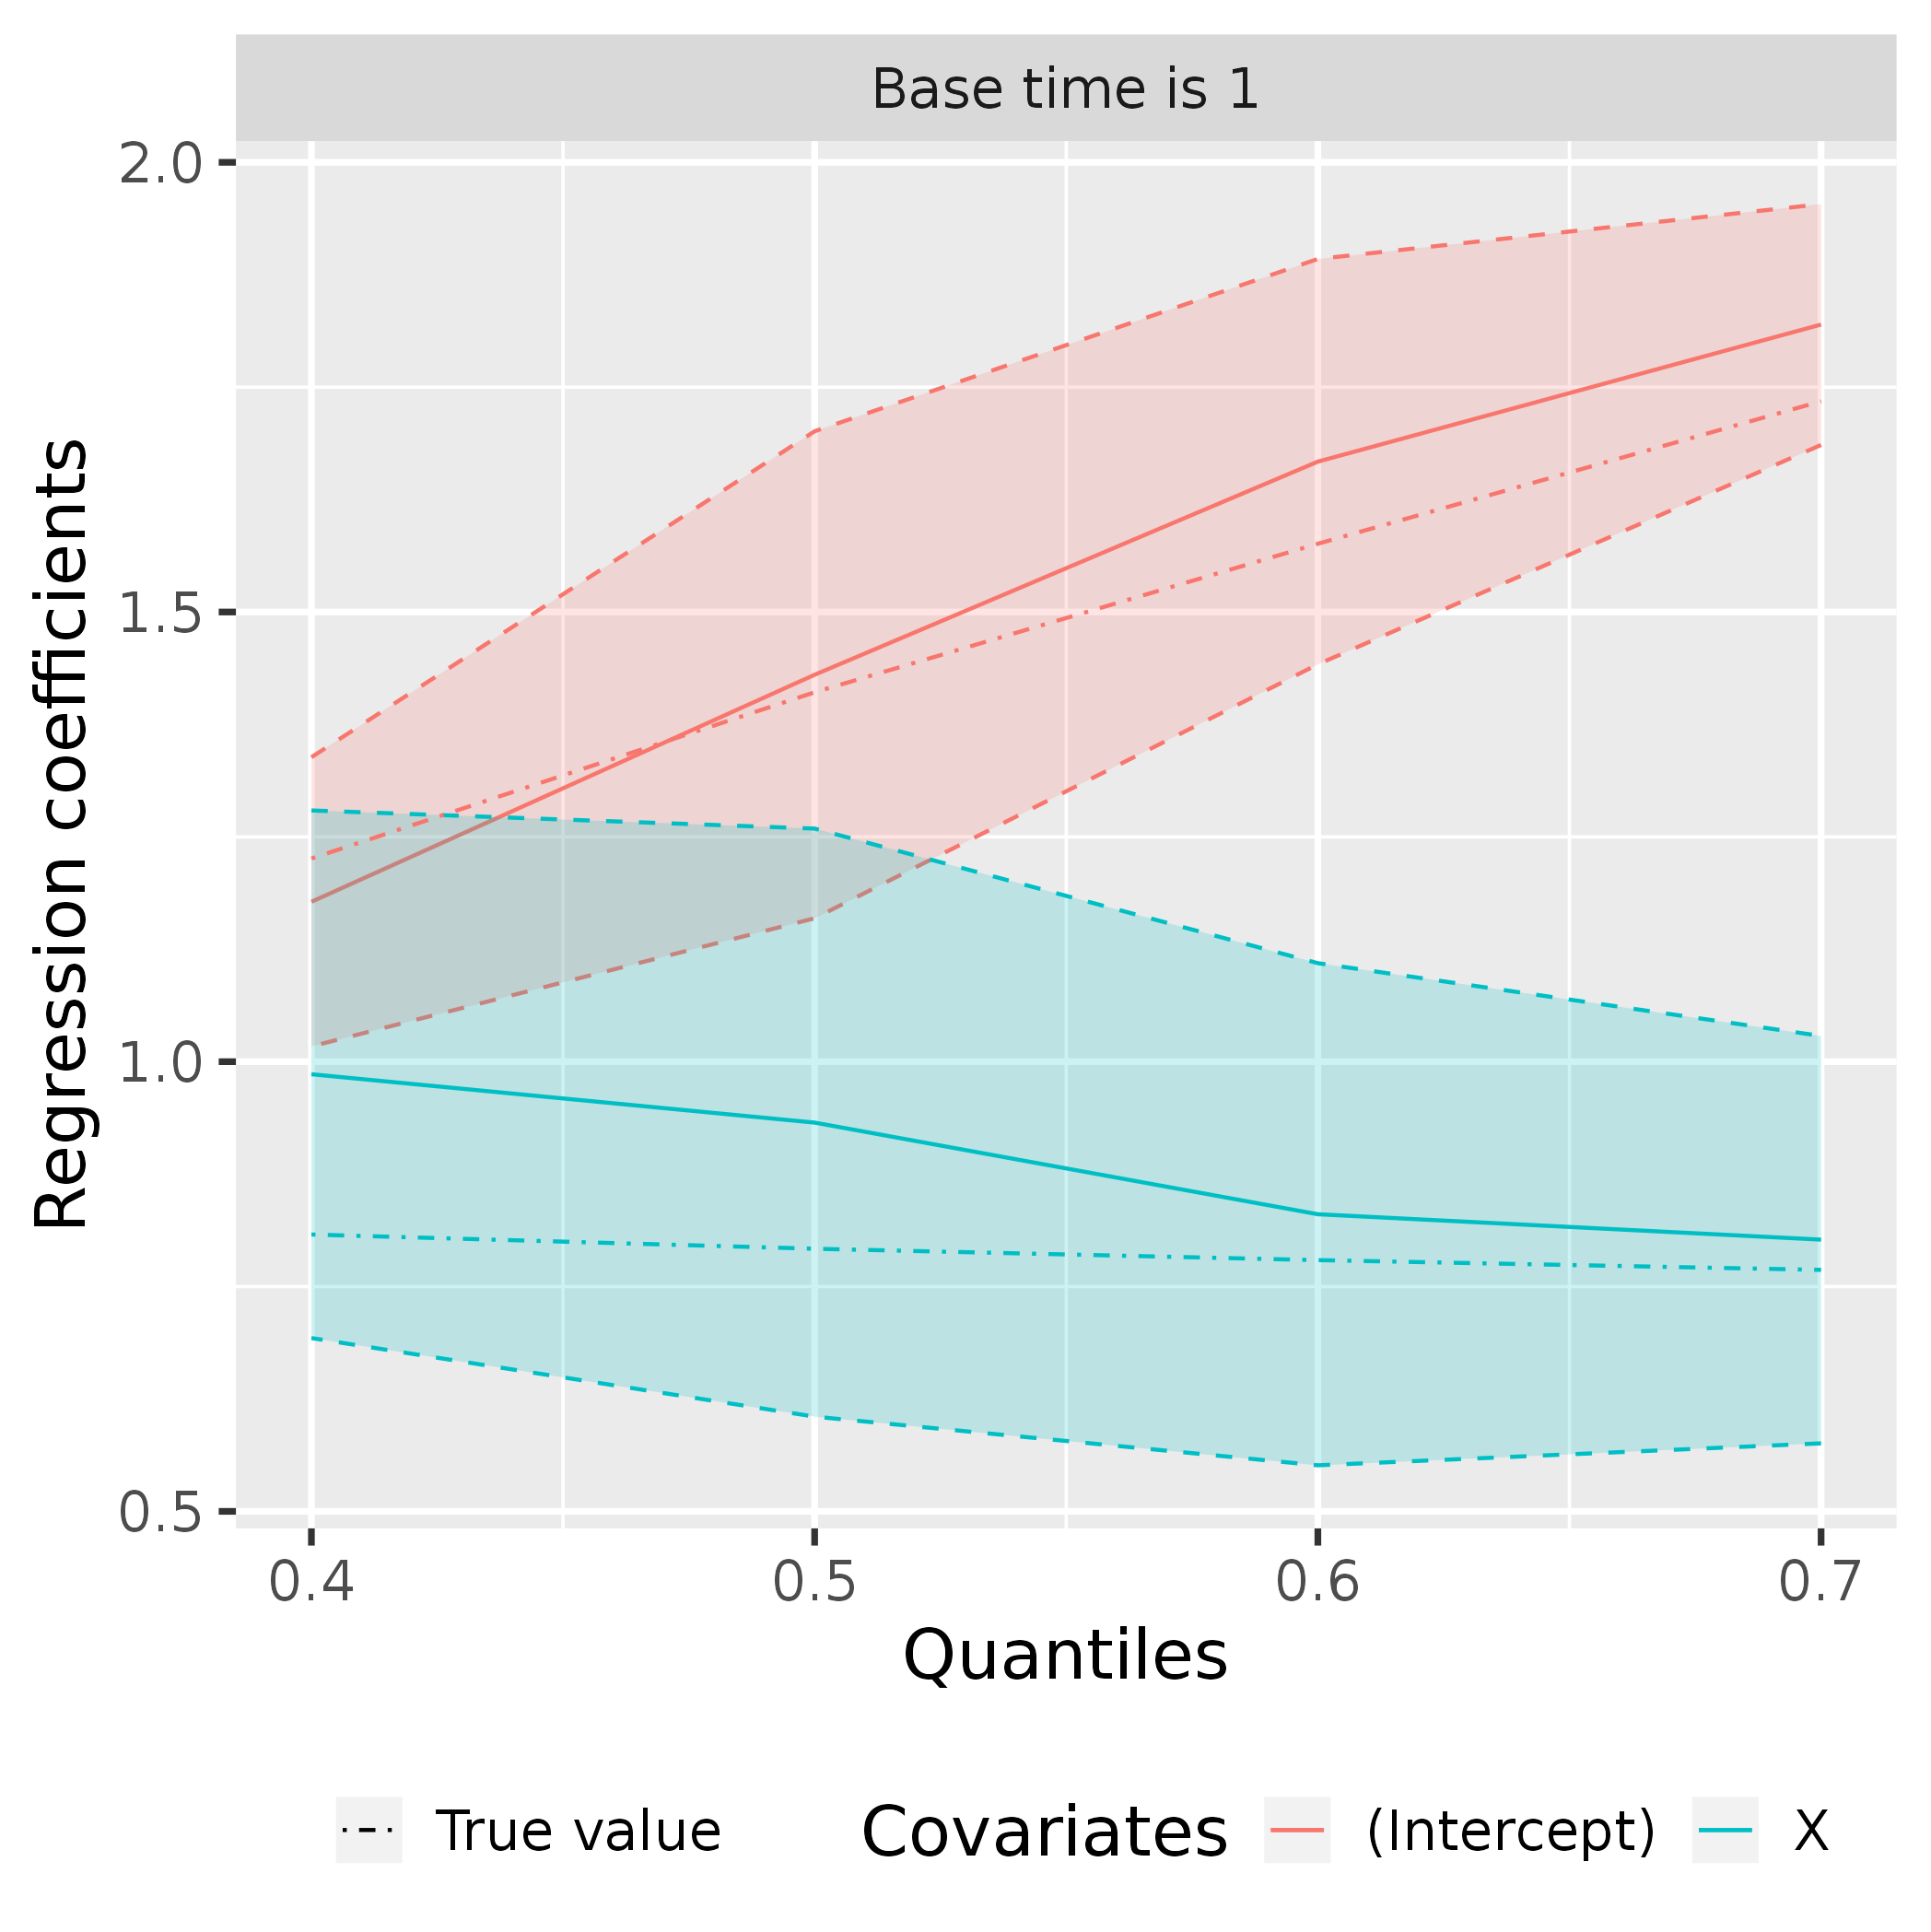
\includegraphics[width = 1.0\textwidth]{simulation_smooth_quantile.png}
    \caption{Plot for $Q\in\{0.4, \ldots, 0.7\}$ at $t_0 = 1$}    
    \label{fig:simulation_quantile}
%  }
  \end{subfigure}
  \hfill
  \begin{subfigure}[b]{0.47\linewidth}
%  \subfigure[Plot for $t_0\in\{1, \ldots, 3\}$ at $Q = 0.5$.]{
    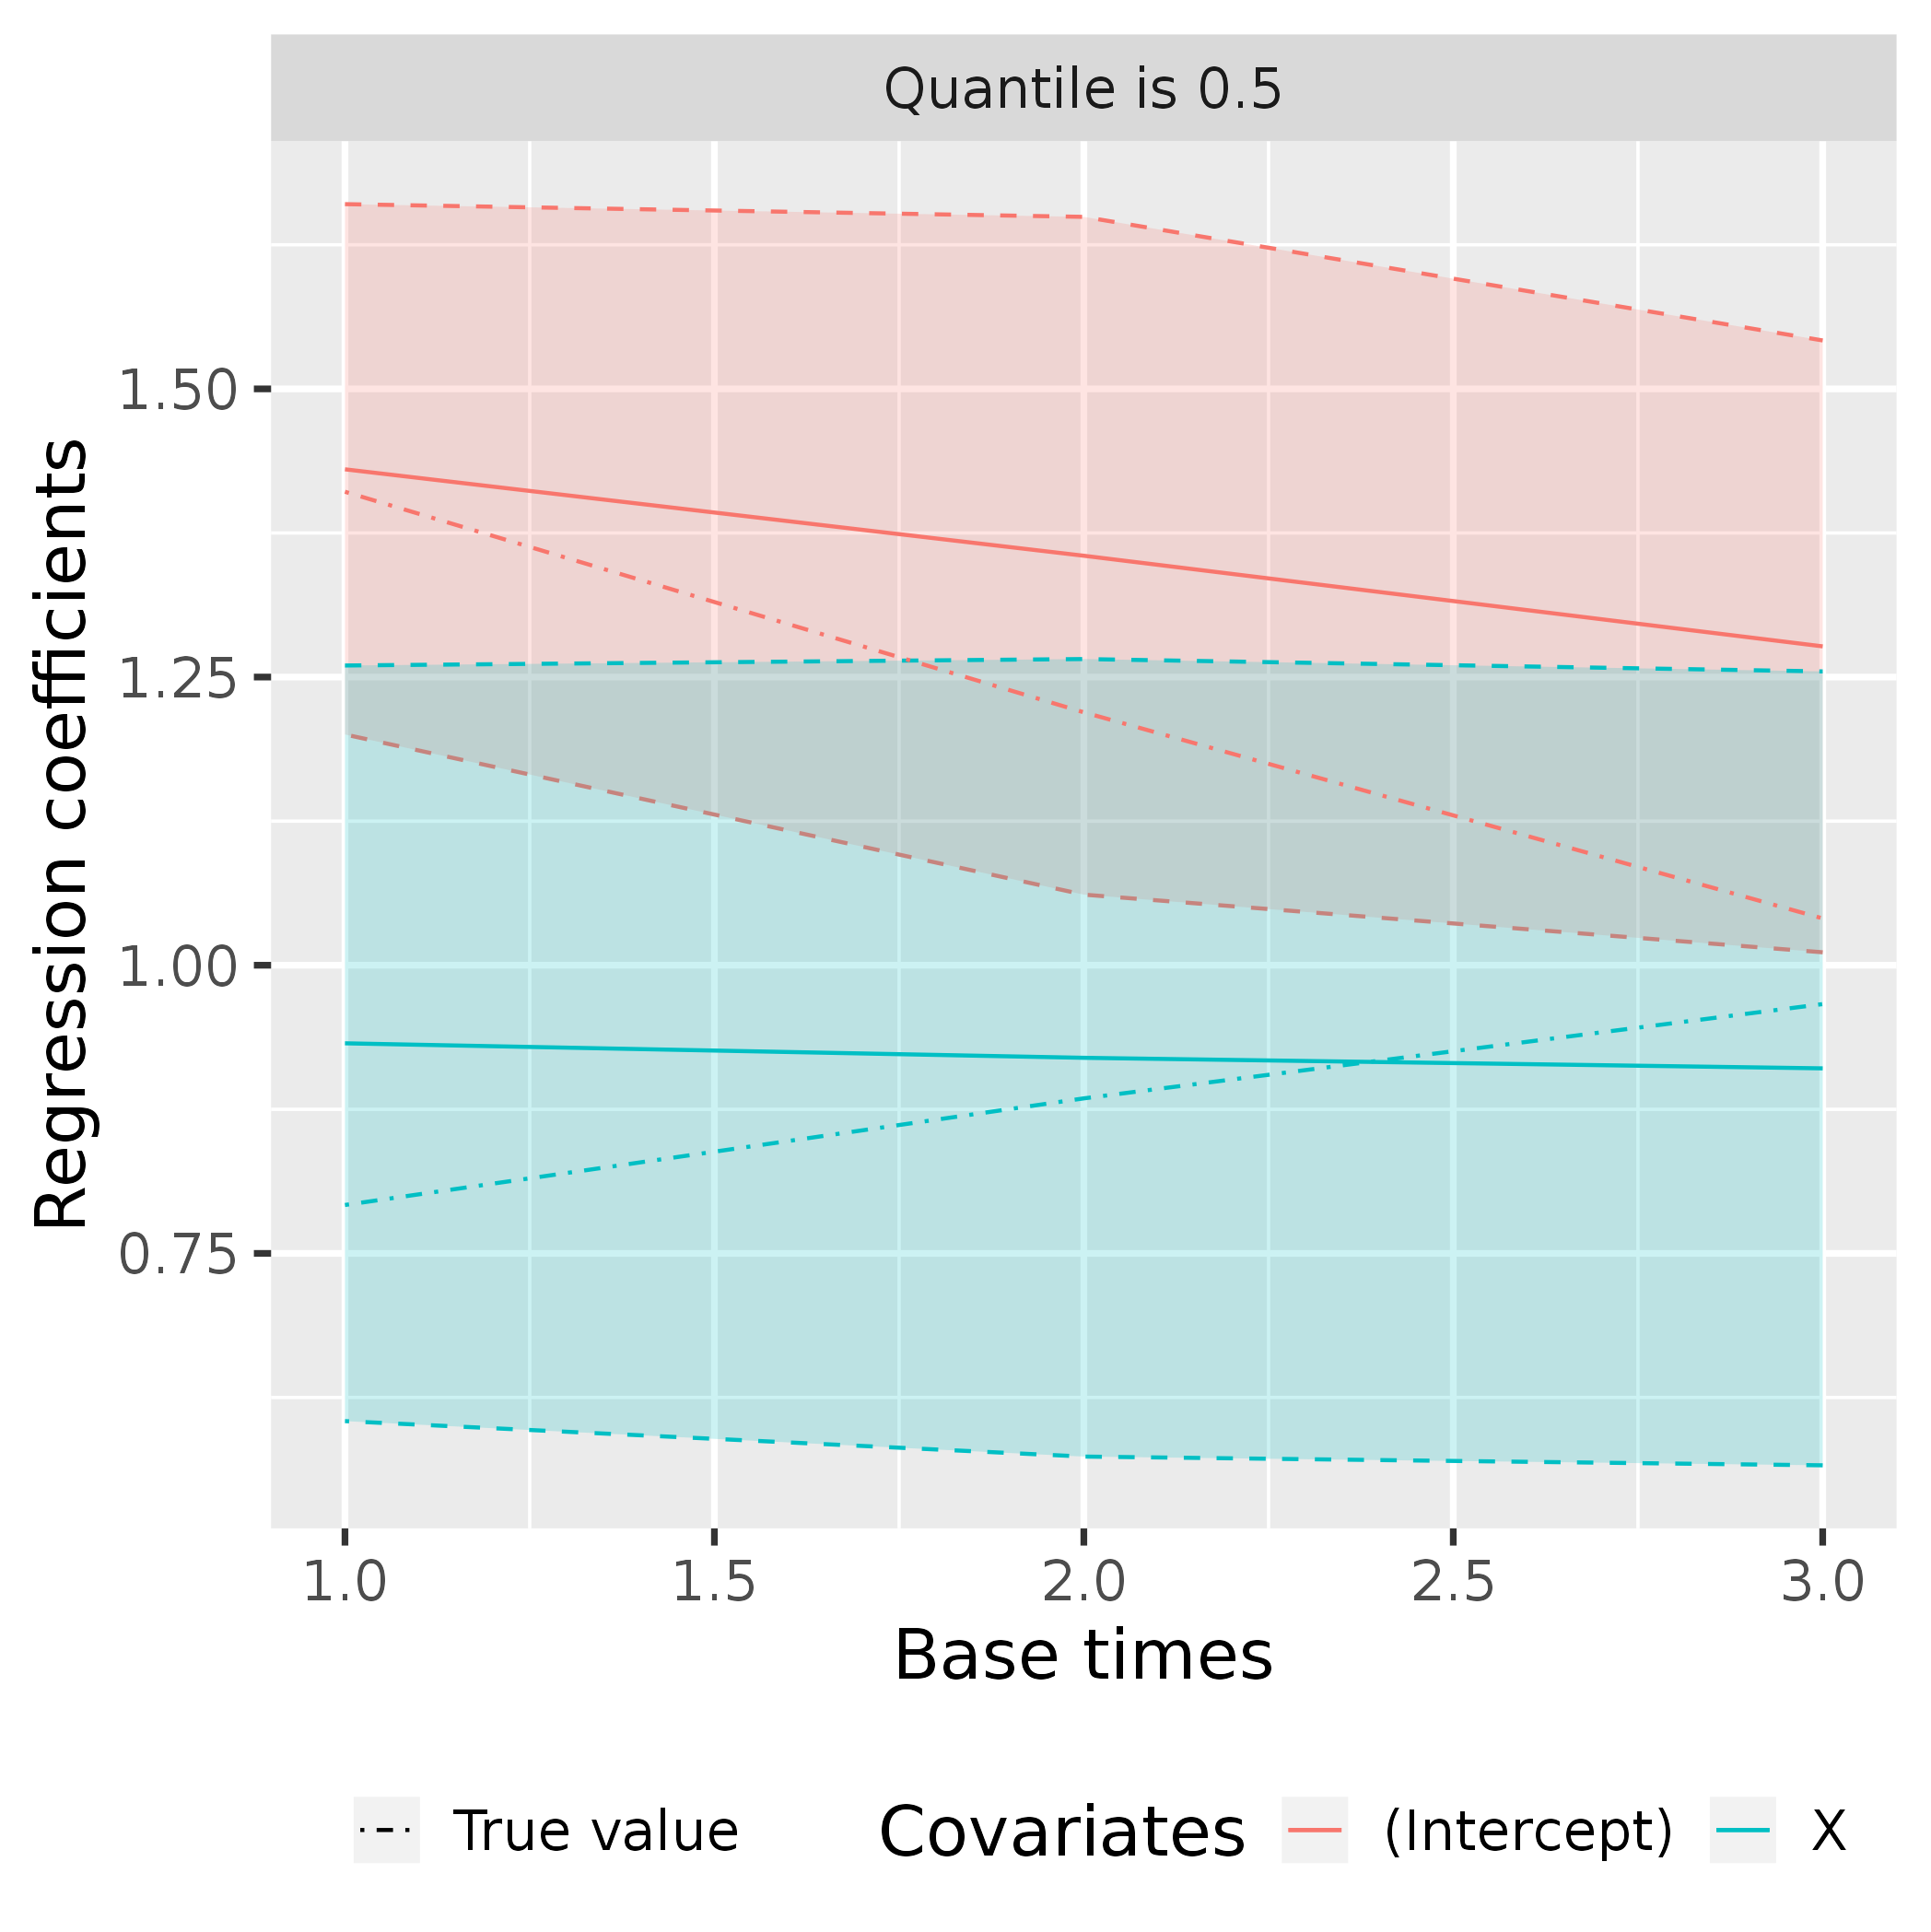
\includegraphics[width = 1.0\textwidth]{simulation_smooth_t0.png}
    \caption{Plot for $t_0\in\{1, \ldots, 3\}$ at $Q = 0.5$}    
    \label{fig:simulation_t0}
%  }
  \end{subfigure}
  \caption{(a) Estimated effects of covariate with the associated $95\%$ pointwise confidence intervals for quantiles ranging from 0.4 to 0.7 at $t_0=1$. Red and blue solid lines are the point estimates of regression parameters for intercept and covariate X, respectively. Similarly, red and blue dotted lines are the upper and lower bounds of $95\%$ pointwise confidence intervals for intercept and covariate X, respectively. 
    (b) Estimated effects of covariate with the associated $95\%$ pointwise confidence intervals for base times ranging from 1 to 3 at $\tau=0.5$. Red and blue solid lines are the point estimates of regression parameters for intercept and covariate X, respectively. Similarly, red and blue dotted lines are the upper and lower bounds of $95\%$ pointwise confidence intervals for intercept and covariate X, respectively.}
  \label{fig:simulation}
\end{figure*}


\subsection{North Central Cancer Treatment Group Lung Cancer Data} \label{subsec:lung}

The North Central Cancer Treatment Group Lung Cancer Data records the survival of patients with advanced lung cancer, 
along with assessments of the patients' performance status measured by both physicians and the patients themselves 
\citep{loprinzi1994prospective}.
The original objective of the study was to ascertain whether descriptive information from a 
patient-completed questionnaire could offer prognostic insights.
The original objective of the study was to determine whether descriptive information from a patient-completed 
questionnaire could provide prognostic information.
However, for this illustration, we focus on how gender and weight loss affect the quantiles of residual life 
for patients diagnosed with advanced lung cancer at different time points.
The lung cancer data are publicly available from the \CRANpkg{survival} package \citep{survivalpackage} as \code{lung}.
The following code displays the structure of the \code{lung} dataset with variables of interest.

\begin{example}
  > data(cancer, package = "survival")
  > str(subset(lung, select = c(time, status, sex, wt.loss)))
  'data.frame':	228 obs. of  4 variables:
  $ time   : num  306 455 1010 210 883 ...
  $ status : num  2 2 1 2 2 1 2 2 2 2 ...
  $ sex    : num  1 1 1 1 1 1 2 2 1 1 ...
  $ wt.loss: num  NA 15 15 11 0 0 10 1 16 34 ...
\end{example}
% \input{codes/cancer0}

The \code{lung} data contains 228 patients whose observed survival times in days and 
censoring status (1 = censored, 2 = dead) are recorded in the \code{time} and the \code{status} columns, 
respectively.
Although the censoring status in this dataset is not recorded in the typical 0-1 fashion,
the \code{Surv()} function is still applicable to create the corresponding ``\code{Surv}" object.
The \code{lung} data yields a censoring rate of $27.6\%$ with a median survival time of 310 days. 
The covariates of interest are gender (\code{sex = 1} if male, \code{sex = 2} if female) and 
weight loss (\code{wt.loss}).
In the following, we use the proposed semiparametric quantile regression models to assess 
the gender and standardized weight loss effects on different quantiles of residual life at different base times.


We first model the median residual life (\code{Q = 0.5}) when the base time is one month (\code{t0 = 30}).
Since the estimated median survival times for combined lung cancers are typically less than one year, 
with a range of 8 to 13 months \citep{siegel2021cancer}, 
setting the base time at one month provides insight into how gender and weight loss impact the residual time 
in early follow-up. 
In the following, we obtain the regression coefficient estimates using the induced smoothing functions and 
the corresponding variance estimate with the partial multiplier bootstrap approach.

\begin{example}
  > lung$male <- factor(lung$sex, 1:2, c("Male", "Female"))
  > lung$std.wt.loss <- scale(lung$wt.loss)
  > fit1 <- qris(Surv(time, status) ~ male + std.wt.loss,
  +              data = lung, t0 = 30, Q = .5, nB = 100,
  +              method = "smooth", se = "pmb")
  > summary(fit1)
  Call:
  qris(formula = Surv(time, status) ~ male + std.wt.loss,
  data = lung, t0 = 30, Q = 0.5, nB = 100, method = "smooth", 
  se = "pmb")

  qris Estimator
                 estimate std.Error z.value p.value    
  (Intercept)      5.5611    0.0950  58.550  <2e-16 ***
  maleFemale       0.4804    0.1805   2.661  0.0078 ** 
  std.wt.loss     -0.0731    0.0837  -0.874  0.3824    
  ---
  Signif. codes:  0 ‘***’ 0.001 ‘**’ 0.01 ‘*’ 0.05 ‘.’ 0.1 ‘ ’ 1
\end{example}
% \input{codes/fitcancer1}

Subjects with missing values (in any of the variables relevant for the modeling task) 
are automatically removed when \code{qris()} is called. 
The estimated intercept implies that the median residual life for patients who have survived up to 30 days 
is $\exp(5.5611) = 260.1$ days for a male with an average weight loss.
More interestingly, the summary shows that the gender effect is statistically significant at the 0.05 significance level, 
indicating that a female patient is expected to have a median residual life at 30 days that is $\exp(0.4804) = 1.617$
times that of a male patient with the same weight loss.
The effect of the weight loss is not statistically significant at the 0.05 level.
In addition to \code{summary()}, important statistics such as the coefficient and variance estimates can be extracted by 
\code{S3} methods \code{coef()} and \code{vcov()}, respectively.

\begin{example}
  > coef(fit1)
  (Intercept)    maleFemale    std.wt.loss 
  5.56111984     0.48044228    -0.07307635 
  > vcov(fit1)
                 (Intercept)   maleFemale    std.wt.loss 
  (Intercept)    0.009021459 -0.010944549   -0.003074041
  maleFemale    -0.010944549  0.032594288    0.002847148
  std.wt.loss   -0.003074041  0.002847148    0.006998314
\end{example}
% \input{codes/s3fit1}
Moreover, the corresponding 95\% Wald-type confidence interval can be printed by applying 
the \code{confint()} function to the \class{qris} object.
\begin{example}
  > confint(fit1)
                    2.5 %     97.5 %
  (Intercept)   5.3749598 5.74727989
  maleFemale    0.1265926 0.83429199
  std.wt.loss  -0.2370390 0.09088626
\end{example}
% \input{codes/cifit1}

The \code{update()} function can be conveniently applied to update existing \class{qris} objects. 
The following examples update the \code{method} and \code{se} arguments from \code{fit1}.
The updated results yield similar coefficient estimates, but the non-smooth procedure (\code{method = "nonsmooth"}) 
yields slightly greater standard error estimates.
\begin{example}
  > summary(fit2 <- update(fit1, method = "nonsmooth", se = "fmb"))
  Call:
  qris(formula = Surv(time, status) ~ male + std.wt.loss,
  data = lung, t0 = 30, Q = 0.5, nB = 100, method = "nonsmooth", 
  se = "fmb")

  qris Estimator
               estimate std.Error z.value p.value    
  (Intercept)    5.5585    0.1132  49.106  <2e-16 ***
  maleFemale     0.4695    0.2015   2.331  0.0198 *  
  std.wt.loss   -0.0668    0.1029  -0.650  0.5159    
  ---
  Signif. codes:  0 ‘***’ 0.001 ‘**’ 0.01 ‘*’ 0.05 ‘.’ 0.1 ‘ ’ 1          
\end{example}
% \input{codes/fitcancer2}

\begin{example}
  > summary(update(fit1, method = "iterative"))
  Call:
  qris(formula = Surv(time, status) ~ male + std.wt.loss,
  data = lung, t0 = 30, Q = 0.5, nB = 100, method = "iterative", 
  se = "pmb")

  qris Estimator
               estimate std.Error z.value p.value    
  (Intercept)    5.5605    0.1016  54.712  <2e-16 ***
  maleFemale     0.4807    0.1626   2.957  0.0031 ** 
  std.wt.loss   -0.0720    0.0903  -0.797  0.4252    
  ---
  Signif. codes:  0 ‘***’ 0.001 ‘**’ 0.01 ‘*’ 0.05 ‘.’ 0.1 ‘ ’ 1
\end{example}
% \input{codes/fitcancer3}

At a lower (\code{Q = 0.25}) and a higher (\code{Q = 0.75}) quantiles, 
the gender effect remains significant at the 0.05 significance level indicating 
female patients are associated with longer lower-quantile and higher-quantile residual life 
than male patients with the same weight loss. 
Among these models, we observed that female patients tend to have higher coefficient estimates 
when fitting higher-quantile residual life. 
While the sign of the estimated regression coefficient for weight loss changes to a negative value 
when considering the lower quantile, the effects remain statistically insignificant for 
both the lower and higher quantiles.


\begin{example}
  > summary(update(fit1, Q = 0.25))
  Call:
  qris(formula = Surv(time, status) ~ male + std.wt.loss,
  data = lung, t0 = 30, Q = 0.25, nB = 100, method = "smooth", 
  se = "pmb")

  qris Estimator
              estimate std.Error z.value p.value    
  (Intercept)   4.9111    0.1034  47.480  <2e-16 ***
  maleFemale    0.4651    0.2041   2.279  0.0227 *  
  std.wt.loss   0.0543    0.0584   0.930  0.3525    
  ---
  Signif. codes:  0 ‘***’ 0.001 ‘**’ 0.01 ‘*’ 0.05 ‘.’ 0.1 ‘ ’ 1
\end{example}
% \input{codes/fitcancer4}
\begin{example}
  > summary(update(fit1, Q = 0.75))
  Call:
  qris(formula = Surv(time, status) ~ male + std.wt.loss,
  data = lung, t0 = 30, Q = 0.75, nB = 100, method = "smooth", 
  se = "pmb")

  qris Estimator
               estimate std.Error z.value p.value    
  (Intercept)    6.0748    0.1063  57.126  <2e-16 ***
  maleFemale     0.5237    0.1487   3.522  0.0004 ***
  std.wt.loss   -0.0171    0.1166  -0.147  0.8835    
  ---
  Signif. codes:  0 ‘***’ 0.001 ‘**’ 0.01 ‘*’ 0.05 ‘.’ 0.1 ‘ ’ 1
\end{example}
% \input{codes/fitcancer5}

We also consider the base time at six months \code{t0 = 180}, 
which enables us to assess gender and weight loss effects in median residual time at a moderate length of follow-up.
The estimated effect for the gender and weight loss increases as $t_0$ increases from $30$ days to $180$ days and 
becomes significant at the 0.05 significant level.
Additionally, the effect of the weight loss seems to be associated with a shorter survival time after 
$180$ days, with a $p$-value of $0.0008$.

\begin{example}
  > summary(update(fit1, t0 = 180))
  Call:
  qris(formula = Surv(time, status) ~ male + std.wt.loss,
  data = lung, t0 = 180, Q = 0.5, nB = 100, method = "smooth", 
  se = "pmb")

  qris Estimator
               estimate std.Error z.value p.value    
  (Intercept)    5.2243    0.0912  57.255  <2e-16 ***
  maleFemale     0.5821    0.1867   3.117  0.0018 ** 
  std.wt.loss   -0.2515    0.0754  -3.337  0.0008 ***
  ---
  Signif. codes:  0 ‘***’ 0.001 ‘**’ 0.01 ‘*’ 0.05 ‘.’ 0.1 ‘ ’ 1
\end{example}
% \input{codes/fitcancer6}

The \class{qris} object is designed to be compatible with \code{S3} methods: \code{predict()} and 
\code{residuals()} functions. 
The following presents the fitted survival times for two hypothetical male and female patients with no weight loss, 
as well as the first five residual values for the dataset.
 \begin{example}
  > lung.new <- data.frame(male = c("Male", "Female"), std.wt.loss = 0)
  > predict(fit2, newdata = lung.new)
         1        2 
  444.9026 289.4422 
  > head(residuals(fit2), 5)
         1          2          3          4          5 
 -20.86127 -575.86127  232.44474 -416.82295 -555.82295 
 \end{example}

To better understand the covariate effects on different quantiles of residual time and across different base times, 
we plot the estimated regression coefficients of the intercept, sex, and weight loss in \code{fit1} and \code{fit2}.
Figures~\ref{fig:realdata_smooth} and~\ref{fig:realdata_nonsmooth} display the estimated regression coefficients when 
\code{method = "smooth"} and \code{method = "nonsmooth"}, respectively, at
different quantiles ranging from 0.2 and 0.5 at $t_0 = 30$ days. 
The \code{plot.qris()} function is currently not available for the iterative estimator. This is mainly due to an extended computation time involved, as indicated by our simulation results, and the nature of plotting that necessitates computations across various quantiles or base times.
As expected, the two plots show very similar patterns. 
We plot the estimated regression coefficients of the intercept, sex, and weight loss for different quantiles in the range
of 0.2 to 0.5 at $t_0= 50$, 60, 70, and 80 days (Figure~\ref{fig:realdata_multi_quantile}), 
as well as for different base times in the range of 50 to 80 days at $\tau=0.2$, 0.3, 0.4, and 0.5 (Figure~\ref{fig:realdata_multi_basetime}). 
The estimation method used is non-iterative induced smoothed estimation (\code{method = "smooth"}). 
In Figure~\ref{fig:realdata_multi_quantile}, 
the estimated intercept increases as the quantile increases (for a given base time). 
The estimated slopes for sex remain largely the same, 
but those for weight loss tend to decrease slightly across different quantiles (for a given base time). 
These patterns remain consistent for different base times.
In Figure~\ref{fig:realdata_multi_basetime}, the estimated intercepts increase as the quantiles increase, 
but with a given quantile, they remain flat across the different base times considered. 
The estimated regression coefficients for the two covariates do not appear to change significantly 
for different base times.

\begin{example}
  > hide <- theme(legend.position = "none")
  > plot(fit1, Qs = 2:5 / 10, byQs = TRUE, ggextra = hide)
  > plot(fit2, Qs = 2:5 / 10, byQs = TRUE, ggextra = hide)
  > plot(fit1, Qs = 2:5 / 10, t0s = 5:8 * 10, byQs = TRUE, ggextra = hide)
  > plot(fit1, Qs = 2:5 / 10, t0s = 5:8 * 10, byQs = FALSE, ggextra = hide)
\end{example}
% \input{codes/plotcancer1}

\begin{figure*}[ht] 
  \centering
    \begin{subfigure}[b]{0.47\linewidth}
%  \subfigure[\code{method = ''smooth''} and \code{se = ''pmb''}]{
    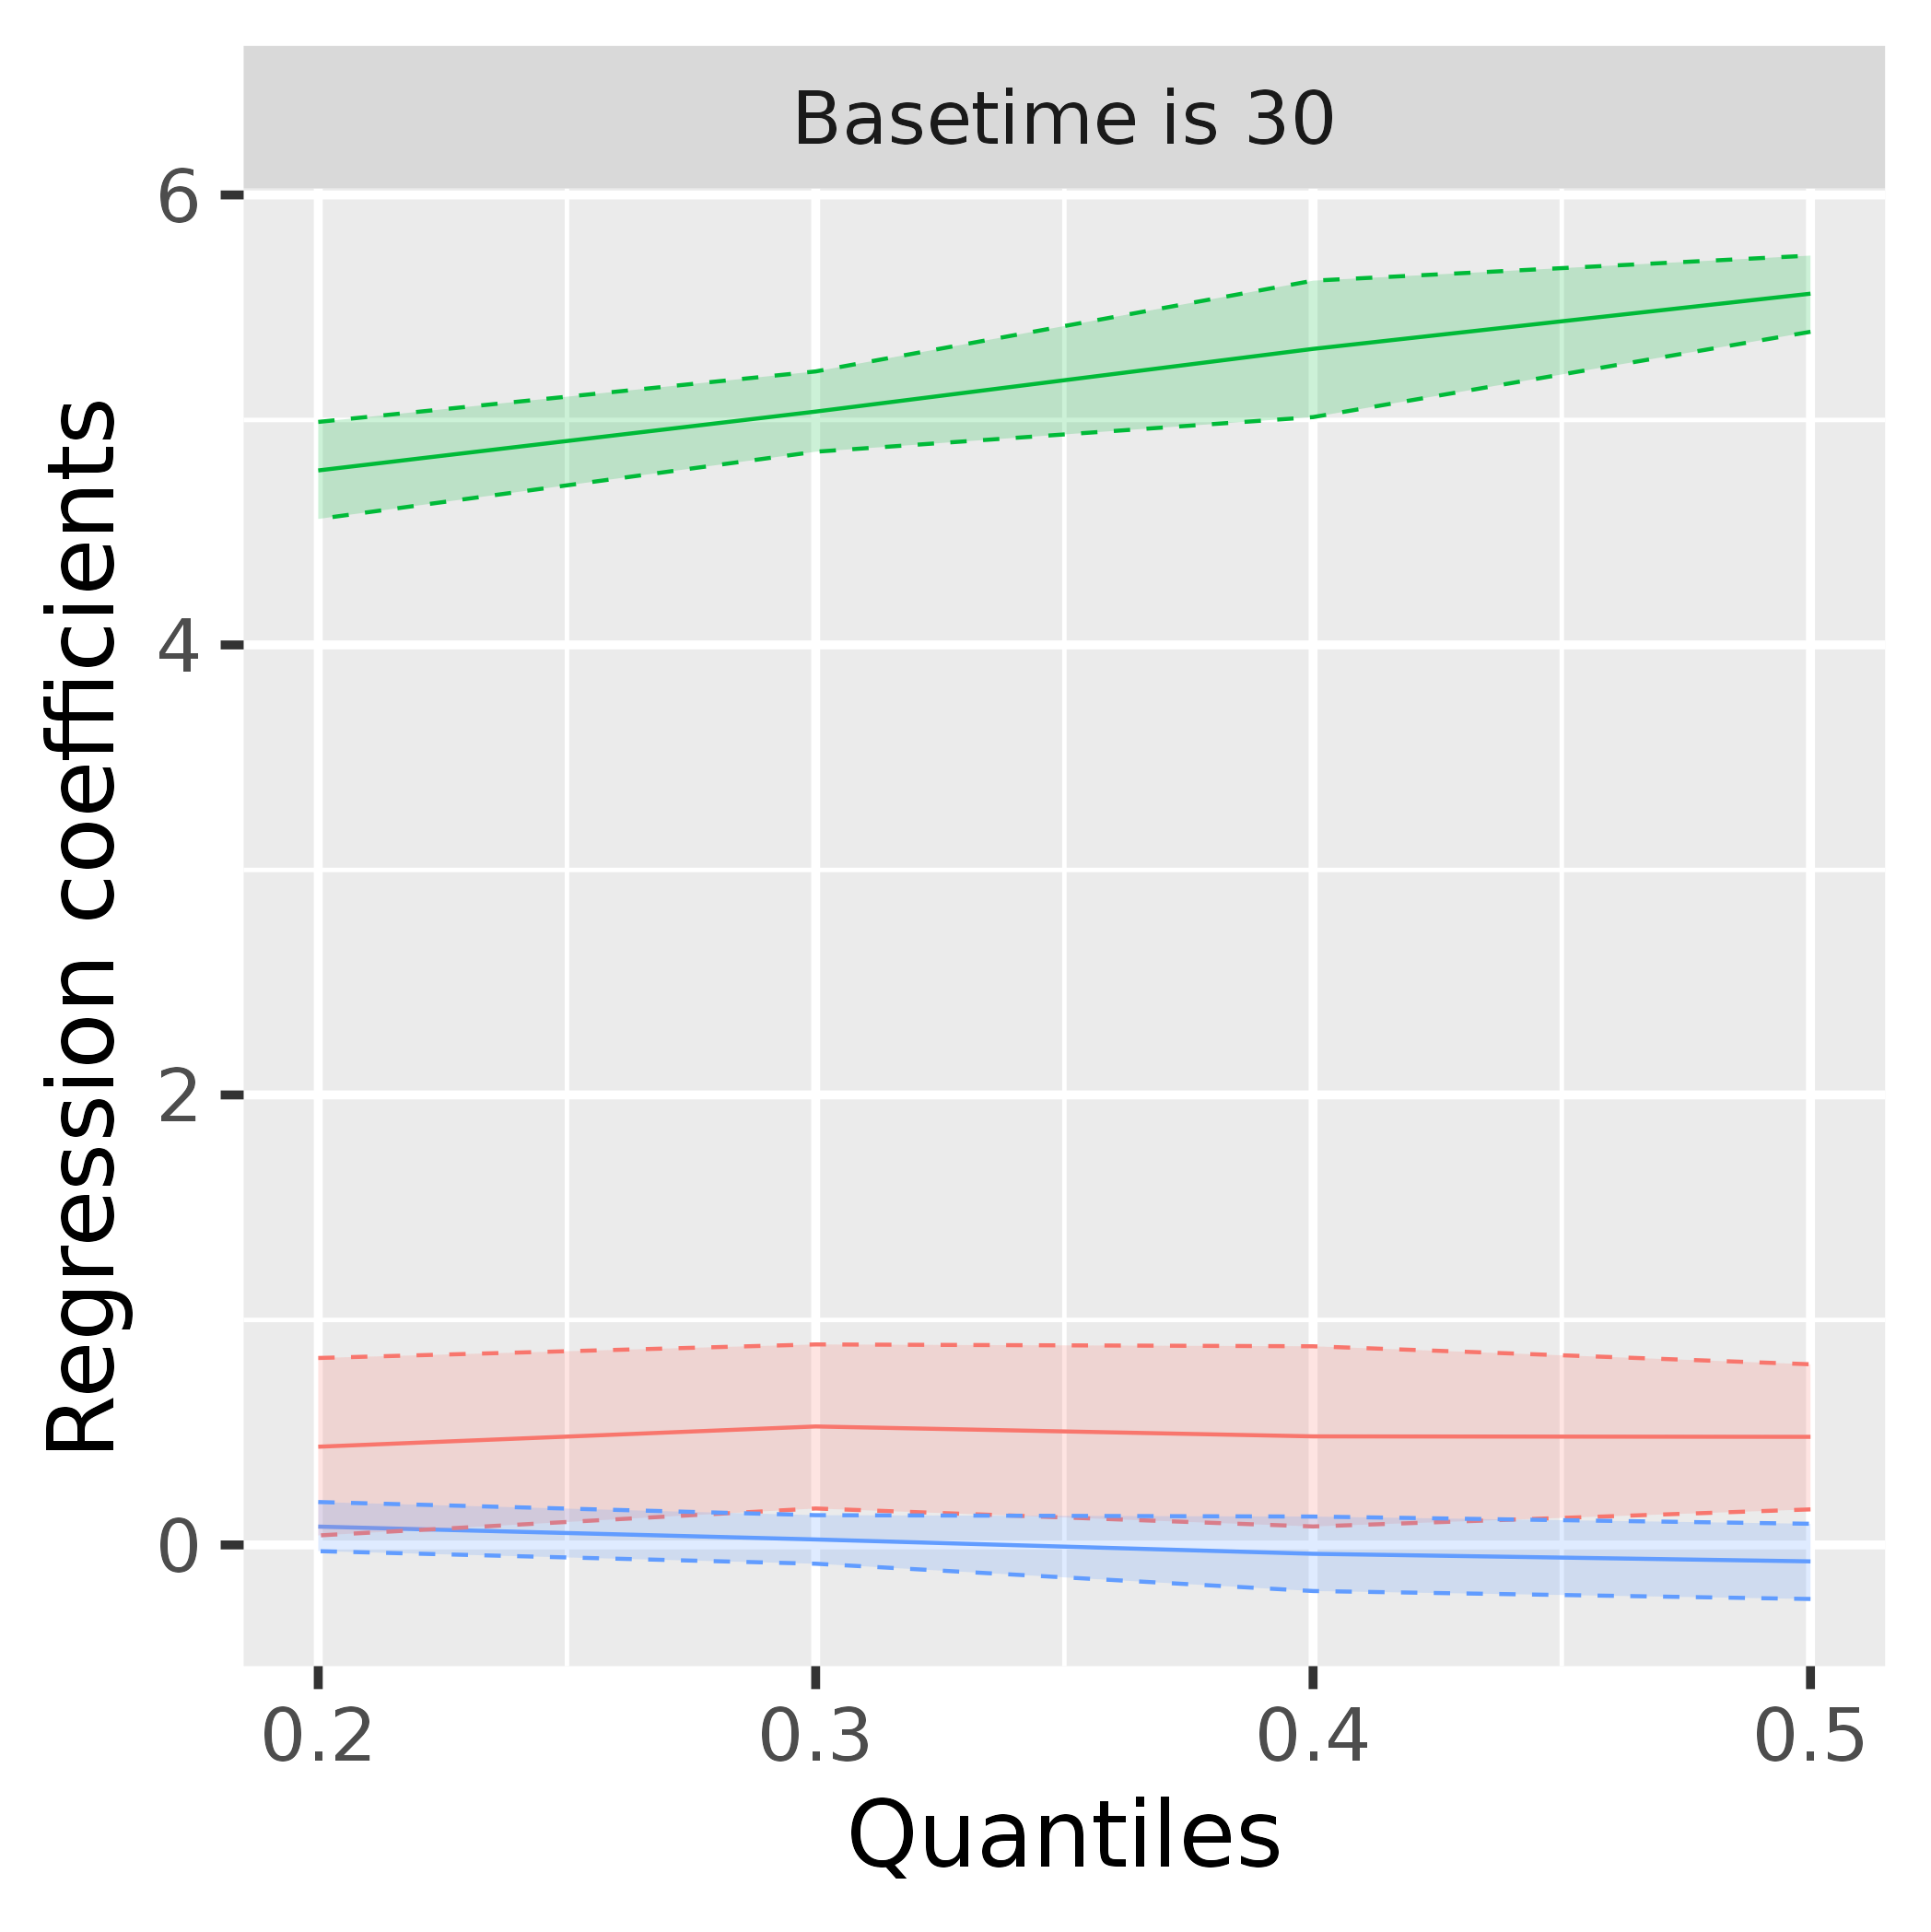
\includegraphics[width = 1.0\textwidth]{realdata_smooth_quantile.png}
    \caption{\code{method = ''smooth''} and \code{se = ''pmb''}}    
    \label{fig:realdata_smooth}
%  }
  \end{subfigure}
%  \hfill
  \begin{subfigure}[b]{0.47\linewidth}
%  \subfigure[\code{method = ''nonsmooth''} and \code{se = ''fmb''}]{
    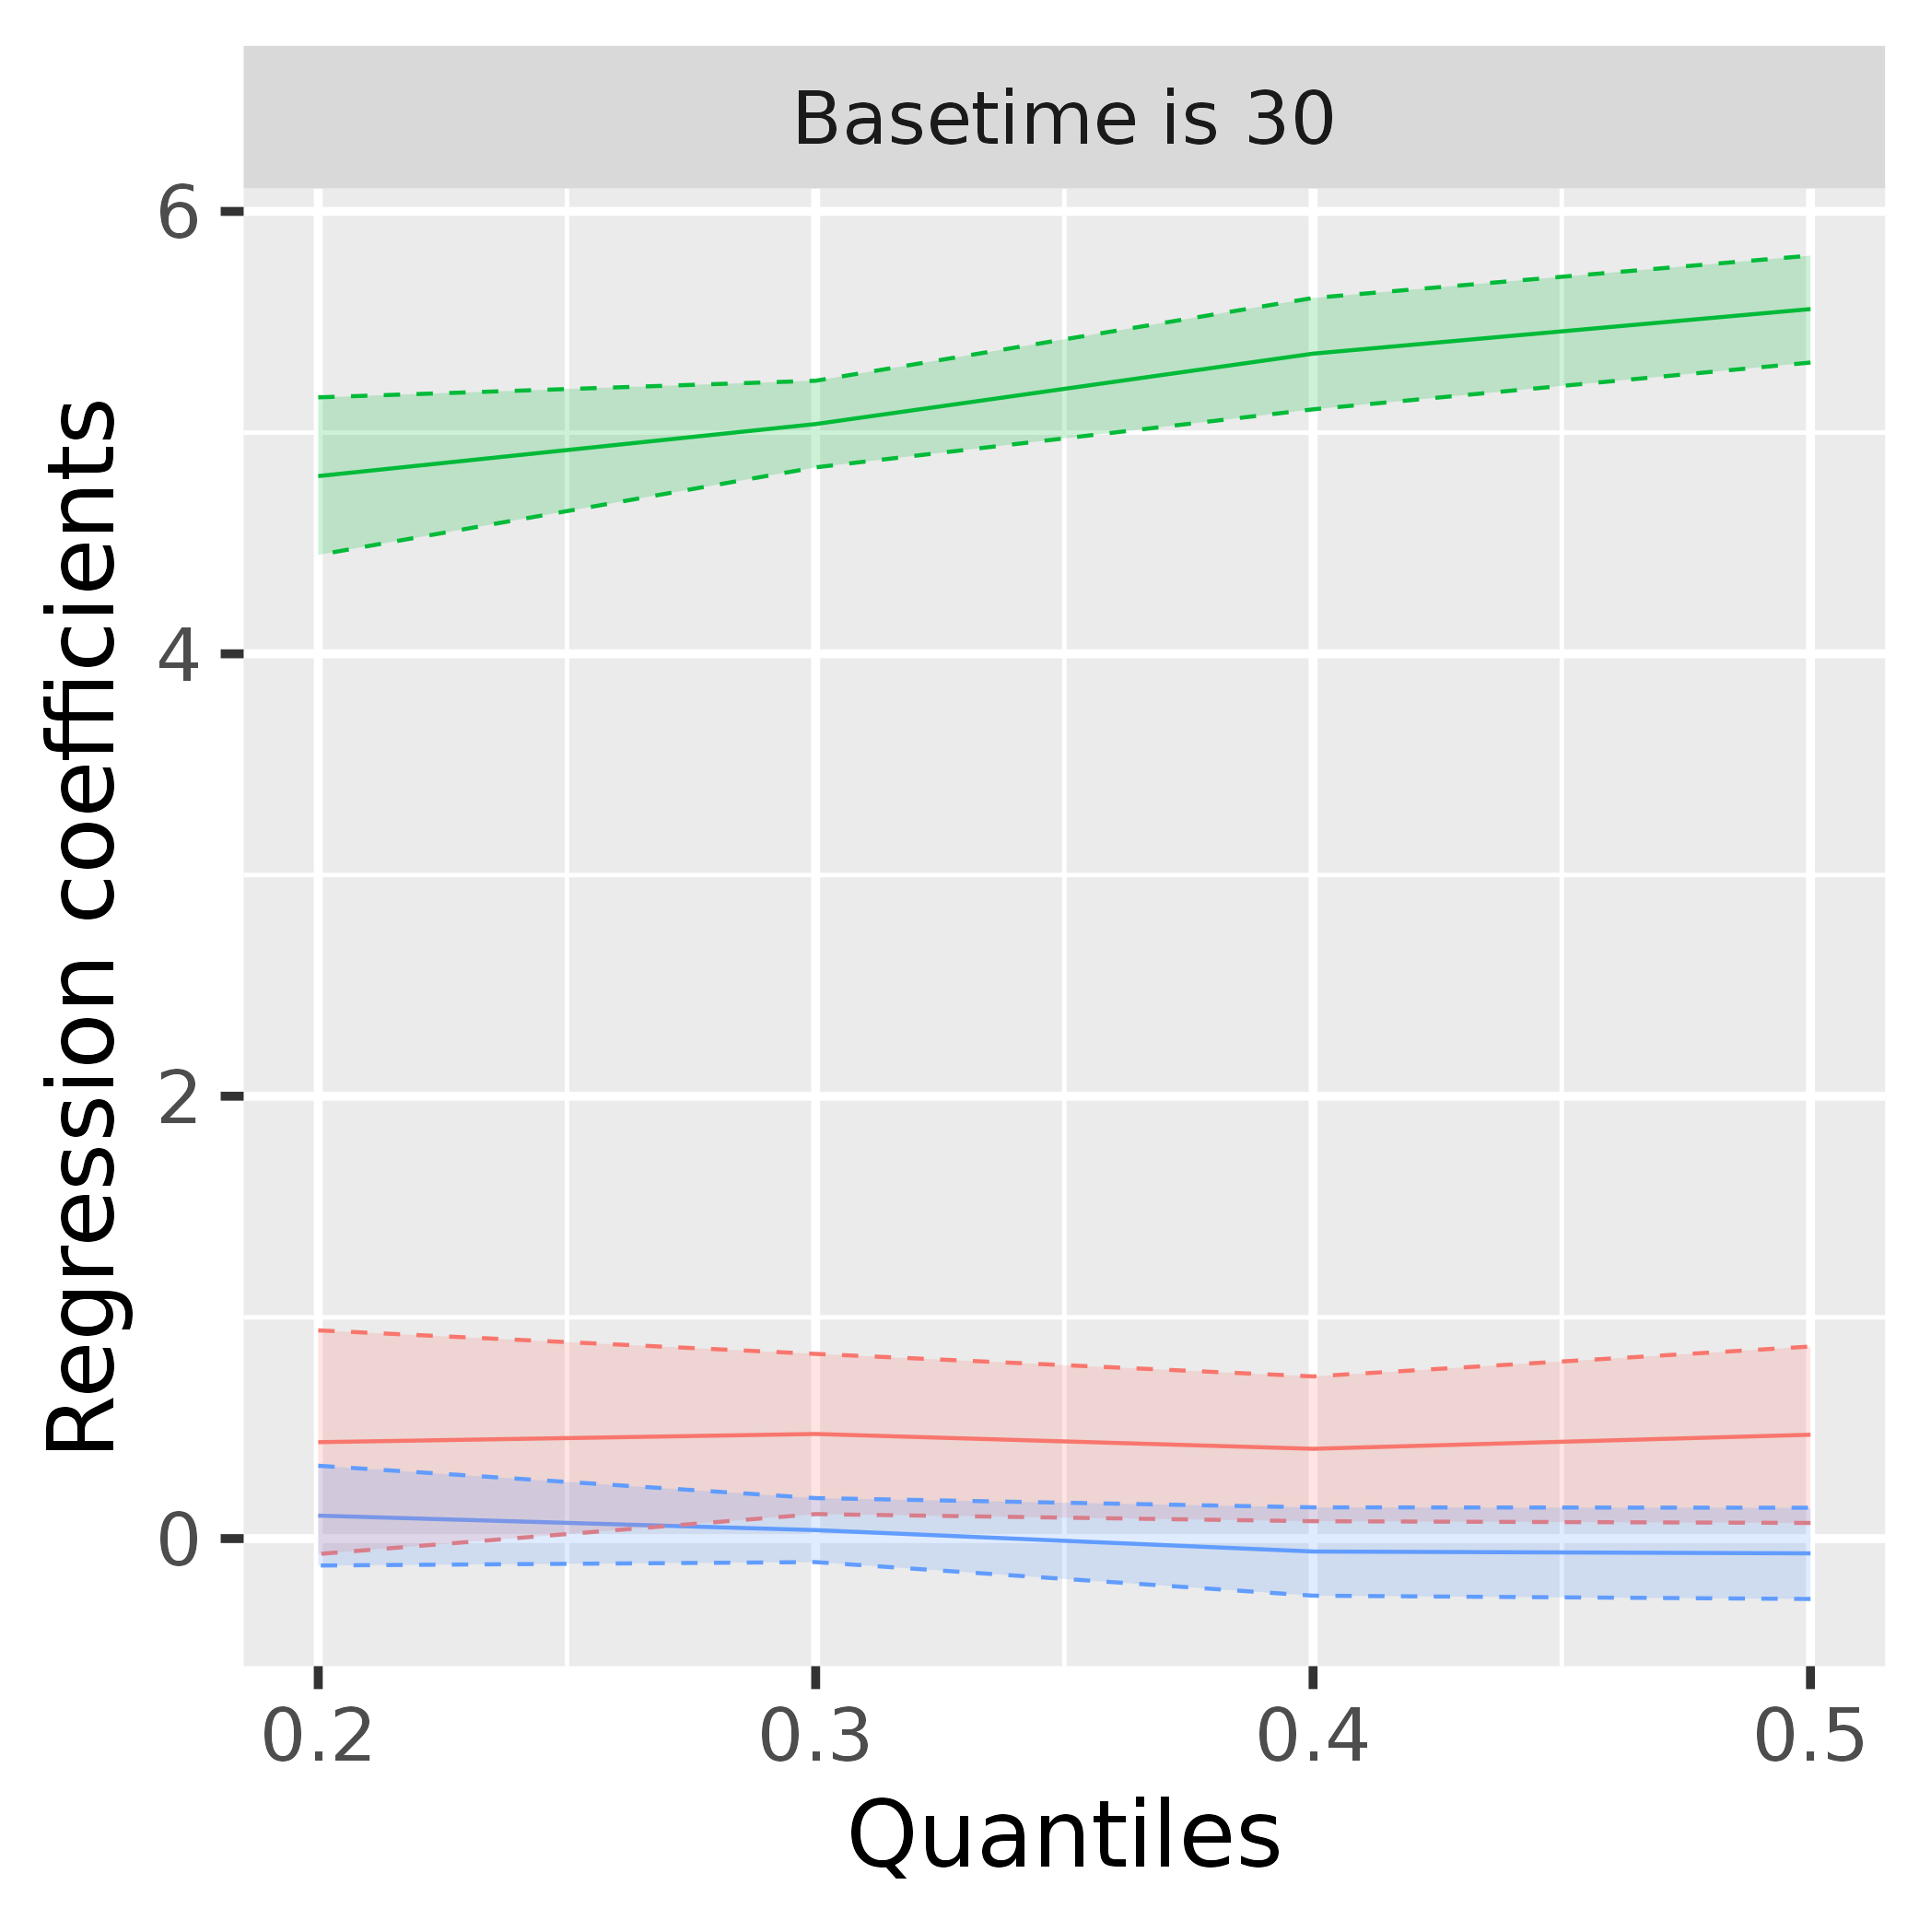
\includegraphics[width = 1.0\textwidth]{realdata_nonsmooth_quantile.png}
    \caption{\code{method = ''nonsmooth''} and \code{se = ''fmb''}}    
    \label{fig:realdata_nonsmooth}
%  }
  \end{subfigure}
 \\[2ex]
  \begin{subfigure}[b]{0.47\linewidth}
%\subfigure[Multiple covariate effect plot against quantiles]{
    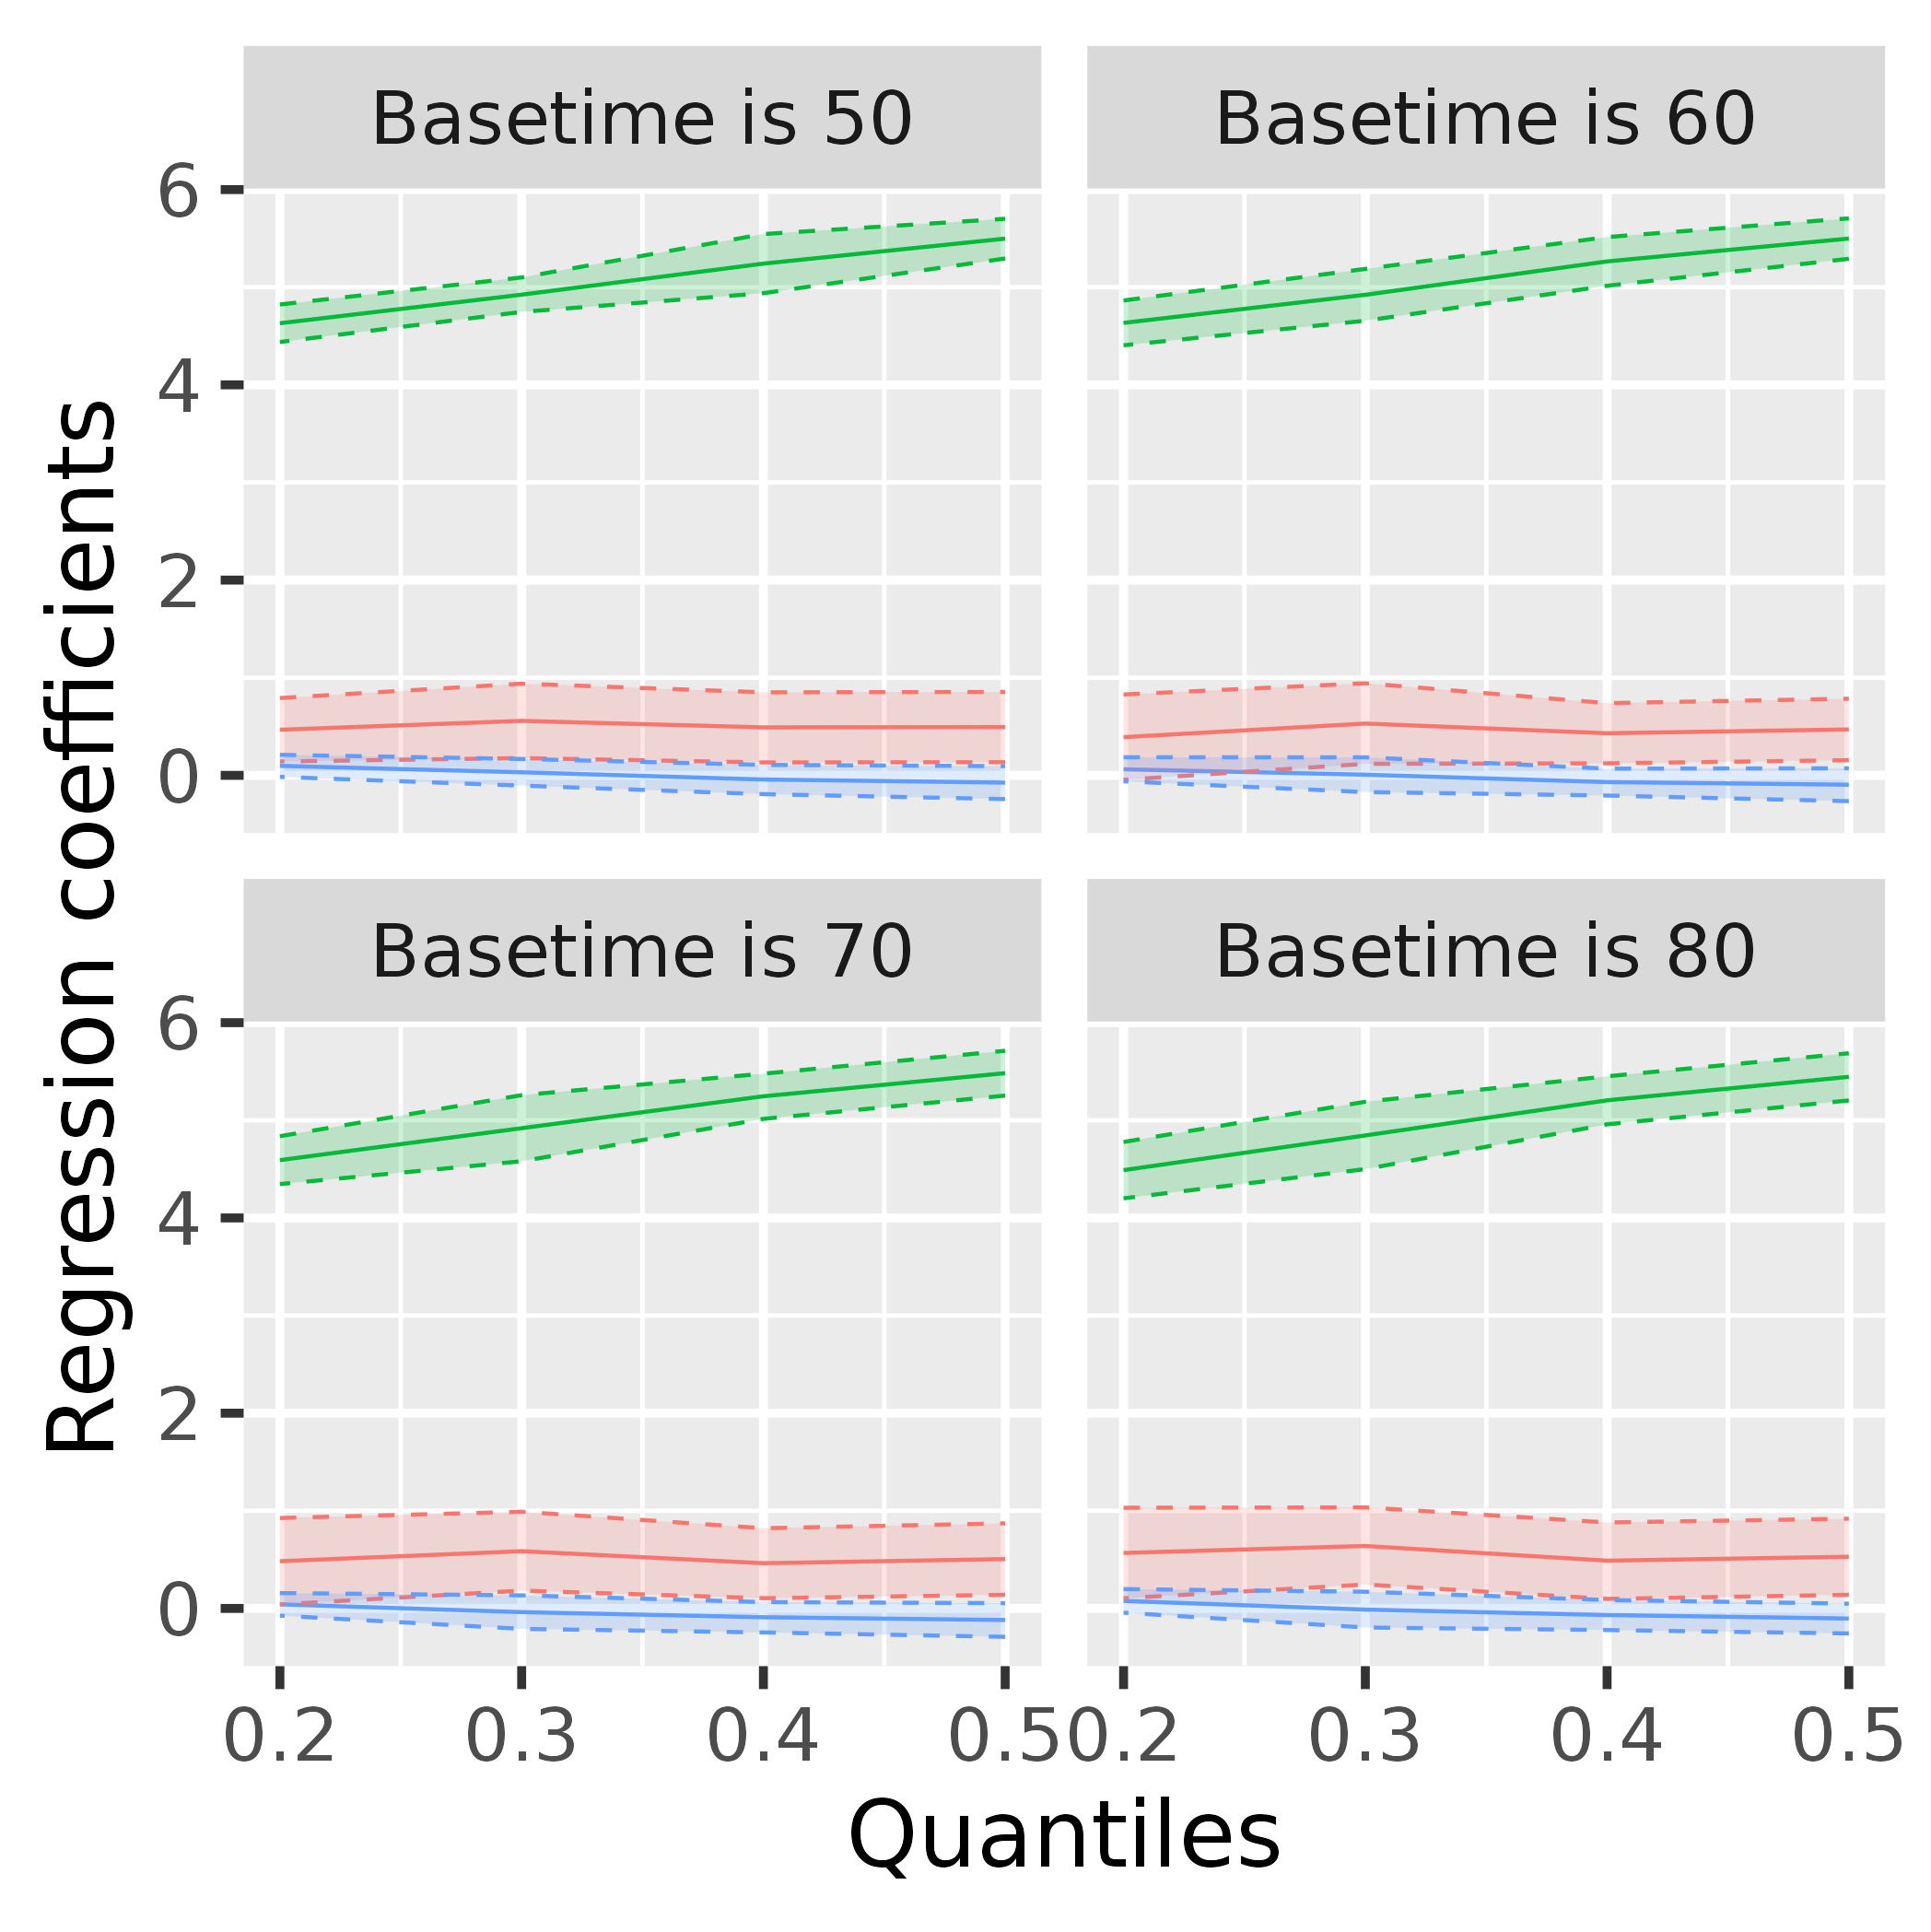
\includegraphics[width = 1.0\textwidth]{realdata_multi_quantile.png}
    \caption{\code{method = ''smooth''} and \code{se = ''pmb''}}    
    \label{fig:realdata_multi_quantile}
%  }
  \end{subfigure}
%  \hfill
  \begin{subfigure}[b]{0.47\linewidth}
%  \subfigure[Multiple covariate effect plot against base time]{
    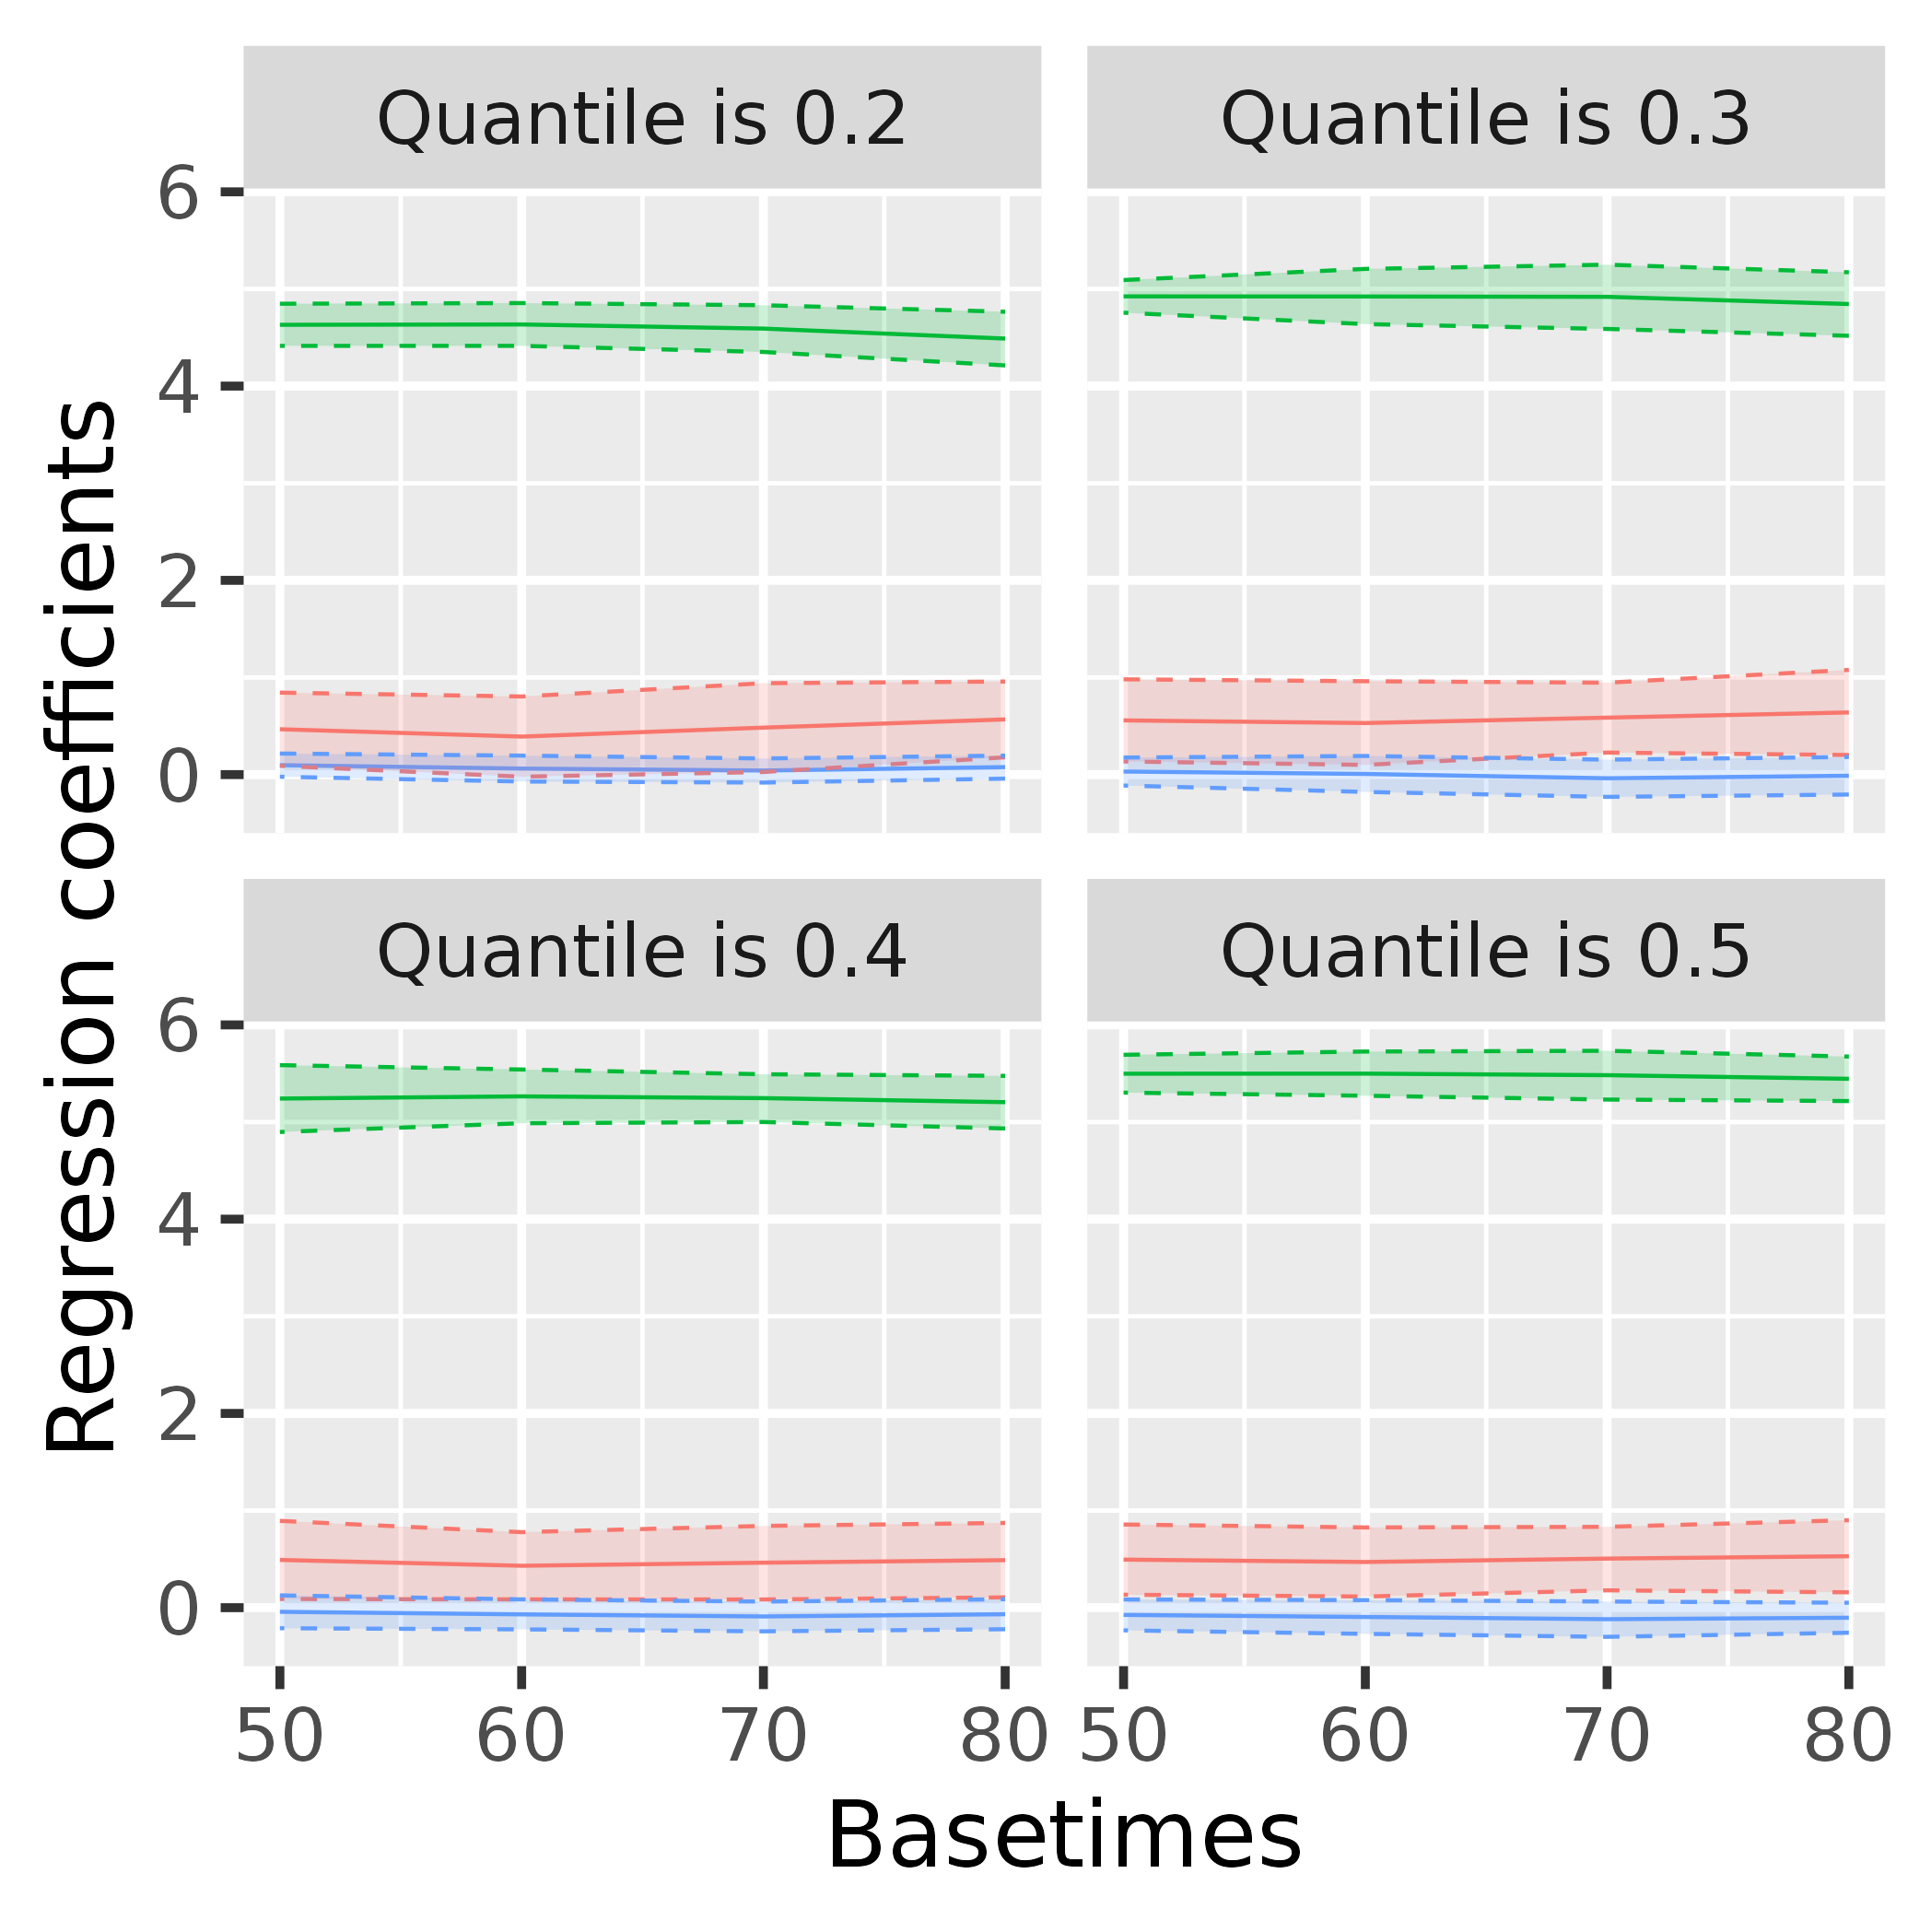
\includegraphics[width = 1.0\textwidth]{realdata_multi_basetime.png}
    \caption{Multiple covariate effect plot against base time}    
    \label{fig:realdata_multi_basetime}
%  }
  \end{subfigure}
  \caption{Green, red and blue lines are the point estimates of regression parameters for 
  intercept, covariate sex and covariate weight loss, respectively. Solid line and dotted line are the point estimates and the upper and lower bounds of $95\%$ pointwise confidence intervals for each regression coefficient.
    (a) \code{method = "smooth"} and \code{se = "pmb"} ($\tau = 0.2, 0.3, 0.4, 0.5, t_0=30$)
    (b) \code{method = "nonsmooth"} and \code{se = "fmb"} ($\tau = 0.2, 0.3, 0.4, 0.5, t_0=30$)
    (c) \code{method = "smooth"} and \code{se = "pmb"} against quantiles ($\tau = 0.2, 0.3, 0.4, 0.5, t_0 = 50, 60, 70, 80$)
    (d) \code{method = "smooth"} and \code{se = "pmb"} against base times ($\tau = 0.2, 0.3, 0.4, 0.5, t_0 = 50, 60, 70, 80$)}
  \label{fig:realdata}
\end{figure*}

%%%%%%%%%%%%%%%%%%%%%%%%%%%% Conclusion %%%%%%%%%%%%%%%%%%%%%%%%%%%%
\section{Conclusion} \label{sec:conclusion}

The purpose of the \CRANpkg{qris} package is to provide a comprehensive tool for fitting quantile regression models on residual life for right-censored survival data, with the aim of promoting widespread dissemination and utilization.
This package implements one estimation method based on non-smooth estimating functions and two estimation methods 
based on their induced smoothed versions.
The non-smooth estimator is calculated through $L_{1}$-type minimization while incorporating the IPCW technique, 
and its variance is calculated using full multiplier bootstrapping. 
The first type of the induced smoothed estimator, a non-iterative version, directly solves estimating functions, 
and its variance can be calculated using either the full multiplier bootstrapping or 
the robust sandwich form with partial multiplier bootstrapping.
As evidenced by the simulation results, this enables one to substantially reduce computing times without sacrificing 
estimation accuracy and stability compared to the original non-smooth function-based method. 
The iterative smoothed estimator has an advantage in obtaining more precise estimates than its non-iterative version, 
although it requires longer computing times. For all these methods, estimates of the regression coefficients and their
variances can be calculated at user-defined quantiles and base times, as long as they are identifiable. 
Additionally, the package provides features for plotting estimates with associated 95\% confidence intervals against 
quantiles and base times using the generic \code{plot} function. 
These plots visualize patterns of estimates at different quantiles and base times, 
helping users to easily grasp the overall picture.
The package \CRANpkg{qris} and its included functions are verified through illustrations using simulated data 
with interpretation of the results demonstrated through a real data application.


Some possible directions for extending our package are as follows. 
Efforts can be made to reduce the computational burden associated with variance estimation, 
which currently accounts for a significant portion of the computing time.
In particular, the iterative-induced smoothed method employs the partial multiplier bootstrap method 
to calculate variance estimates in each iteration. 
Since this method requires multiple iterations, it is crucial to explore more computationally efficient variance
estimation procedures for each iteration to reduce the currently relatively longer computation time. 
One approach is to utilize a closed-form estimation of the mid-part of the sandwich-type variance, 
as discussed in \citet{chiou2014fast, choi2018smoothed}. 
Implementing this direct variance estimation in each iteration is expected to further enhance computation efficiency.
Another direction is to generalize the approaches to allow for the inclusion of sampling weights, 
which is useful for bias correction when failure time data are generated from non-random sampling designs, 
such as case-cohort designs \citep{prentice1986case, chiou2015semiparametric}. 
% To obtain valid parameter estimates under such study designs, the incorporation of sampling weights is a standard approach. 
The current estimating functions implemented in the \CRANpkg{qris} package assume that the data are randomly sampled, 
with sampling weights set to 1."
% Incorporation of sampling weights that can accommodate unequal probabilities of being sampled in the \code{qris} function is a natural direction of future extension.
To the best of our knowledge, there is a lack of model-checking procedures and model-comparison methods 
specifically designed for the non-smooth estimator, 
and a logical next step would be to develop these procedures for subsequent integration into the package.


\bibliography{2022-185_R3}

\address{Kyu Hyun Kim\\
  Department of Statistics and Data Science \emph{and} Department of Applied Statistics\\
  Yonsei University\\
  50 Yonsei-ro, Seodaemun-gu, Seoul\\
  Republic of Korea\\
  \email{kyuhyunkim07@yonsei.ac.kr}}

\address{Sangwook Kang\\
  Department of Statistics and Data Science \emph{and} Department of Applied Statistics\\
  Yonsei University\\
  50 Yonsei-ro, Seodaemun-gu, Seoul\\
  Republic of Korea\\
  \email{kanggi1@yonsei.ac.kr}}

\address{Sy Han Chiou\\
  Department of Statistics and Data Science\\
  Southern Methodist University\\
  P.O. Box 750332, Dallas, TX\\ USA\\
  \email{schiou@smu.edu}\\
  \url{https://www.sychiou.com/}}

\end{article}
\end{document}
